\documentclass[12pt,a4paper]{article}
\usepackage[utf8]{inputenc}
\usepackage[english,swedish]{babel}
\usepackage[pdftex,bookmarks=true]{hyperref} 	% Fixar klickbara länkar i pdf
\usepackage{graphicx} 					% Grafik
\graphicspath{{../includes/figures/}}
\setlength{\parskip}{10pt plus 1pt minus 1pt}
\usepackage{mathtools}					% Matematiska formler
\usepackage{color}						% Färger
\usepackage[usenames,dvipsnames,svgnames,table]{xcolor}
\usepackage{eurosym}
\usepackage{pdfpages} % För att kunna lägga till PDF
\usepackage{lscape}

\begin{document}

%%%%%%%%%%%%%%%%%%%%%%%%%%%%%%%%%%%%%%%%%
% University Assignment Title Page 
% LaTeX Template
%
% This template has been downloaded from:
% http://www.latextemplates.com
%
% Original author:
% WikiBooks (http://en.wikibooks.org/wiki/LaTeX/Title_Creation)
% 
% Instructions for using this template:
% This title page is presently capable of being compiled as is. This is not 
% useful for including it in another document. To do this, you have two options: 
%
% 1) Copy/paste everything between \begin{document} and \end{document} 
% starting at \begin{titlepage} and paste this into another LaTeX file where you 
% want your title page.
% OR
% 2) Remove everything outside the \begin{titlepage} and \end{titlepage} and 
% move this file to the same directory as the LaTeX file you wish to add it to. 
% Then add %%%%%%%%%%%%%%%%%%%%%%%%%%%%%%%%%%%%%%%%%
% University Assignment Title Page 
% LaTeX Template
%
% This template has been downloaded from:
% http://www.latextemplates.com
%
% Original author:
% WikiBooks (http://en.wikibooks.org/wiki/LaTeX/Title_Creation)
% 
% Instructions for using this template:
% This title page is presently capable of being compiled as is. This is not 
% useful for including it in another document. To do this, you have two options: 
%
% 1) Copy/paste everything between \begin{document} and \end{document} 
% starting at \begin{titlepage} and paste this into another LaTeX file where you 
% want your title page.
% OR
% 2) Remove everything outside the \begin{titlepage} and \end{titlepage} and 
% move this file to the same directory as the LaTeX file you wish to add it to. 
% Then add %%%%%%%%%%%%%%%%%%%%%%%%%%%%%%%%%%%%%%%%%
% University Assignment Title Page 
% LaTeX Template
%
% This template has been downloaded from:
% http://www.latextemplates.com
%
% Original author:
% WikiBooks (http://en.wikibooks.org/wiki/LaTeX/Title_Creation)
% 
% Instructions for using this template:
% This title page is presently capable of being compiled as is. This is not 
% useful for including it in another document. To do this, you have two options: 
%
% 1) Copy/paste everything between \begin{document} and \end{document} 
% starting at \begin{titlepage} and paste this into another LaTeX file where you 
% want your title page.
% OR
% 2) Remove everything outside the \begin{titlepage} and \end{titlepage} and 
% move this file to the same directory as the LaTeX file you wish to add it to. 
% Then add \input{./title_page_1.tex} to your LaTeX file where you want your
% title page.
%
%%%%%%%%%%%%%%%%%%%%%%%%%%%%%%%%%%%%%%%%%

%----------------------------------------------------------------------------------------
%	PACKAGES AND OTHER DOCUMENT CONFIGURATIONS
%----------------------------------------------------------------------------------------

\begin{titlepage}

\newcommand{\HRule}{\rule{\linewidth}{0.5mm}} % Defines a new command for the horizontal lines, change thickness here

\center % Center everything on the page
 
%----------------------------------------------------------------------------------------
%	HEADING SECTIONS
%----------------------------------------------------------------------------------------

\textsc{\LARGE Tekniska högskolan vid \\Linköpings Universitet}\\[1.5cm] % Name
% of your university/college
\textsc{\Large TNE085}\\[0.5cm] % Major heading such as course name
\textsc{\large Projektkurs, CDIO}\\[0.5cm] % Minor heading such as course title

%----------------------------------------------------------------------------------------
%	TITLE SECTION
%----------------------------------------------------------------------------------------

\HRule \\[0.4cm]
{ \huge \bfseries Utveckling av svävare}\\[0.4cm] % Title of your document
\HRule \\[1.5cm]
 
%----------------------------------------------------------------------------------------
%	AUTHOR SECTION
%----------------------------------------------------------------------------------------

\begin{minipage}[t]{0.45\textwidth}
\begin{flushleft} \large

\emph{Gruppmedlemmar:}\\
\setlength{\tabcolsep}{2pt}
\begin{tabular}[]{rl}
Emil & \textsc{Andersson} \\
Jesper &\textsc{Cronborn} \\
Rickard & \textsc{Dahm} \\
Johan & \textsc{Gustafsson} \\
Rikard & \textsc{Israelsson} \\
Viktor & \textsc{Johansson} \\
Daniel & \textsc{Josefsson} \\
Olle & \textsc{Kalered} \\
Jens & \textsc{Moser}
\end{tabular}
%\setlength{\tabcolsep}{6pt}

\end{flushleft}
\end{minipage}
~
\begin{minipage}[t]{0.45\textwidth}
\begin{flushright} \large
\emph{Beställare:} \\
\setlength{\tabcolsep}{2pt}
\begin{tabular}[]{rl}
Fo.ing. Gustav &\textsc{Knutsson} \\
Uadj. Ole &\textsc{Pedersen}
\end{tabular}
\end{flushright}
\end{minipage}\\[4cm]

% If you don't want a supervisor, uncomment the two lines below and remove the section above
%\Large \emph{Author:}\\
%John \textsc{Smith}\\[3cm] % Your name

%----------------------------------------------------------------------------------------
%	DATE SECTION
%----------------------------------------------------------------------------------------

{\large \today}\\[3cm] % Date, change the \today to a set date if you want
% to be precise

%----------------------------------------------------------------------------------------
%	LOGO SECTION
%----------------------------------------------------------------------------------------

%\includegraphics{Logo}\\[1cm] % Include a department/university logo - this will require the graphicx package
 
%----------------------------------------------------------------------------------------

\vfill % Fill the rest of the page with whitespace

\end{titlepage} to your LaTeX file where you want your
% title page.
%
%%%%%%%%%%%%%%%%%%%%%%%%%%%%%%%%%%%%%%%%%

%----------------------------------------------------------------------------------------
%	PACKAGES AND OTHER DOCUMENT CONFIGURATIONS
%----------------------------------------------------------------------------------------

\begin{titlepage}

\newcommand{\HRule}{\rule{\linewidth}{0.5mm}} % Defines a new command for the horizontal lines, change thickness here

\center % Center everything on the page
 
%----------------------------------------------------------------------------------------
%	HEADING SECTIONS
%----------------------------------------------------------------------------------------

\textsc{\LARGE Tekniska högskolan vid \\Linköpings Universitet}\\[1.5cm] % Name
% of your university/college
\textsc{\Large TNE085}\\[0.5cm] % Major heading such as course name
\textsc{\large Projektkurs, CDIO}\\[0.5cm] % Minor heading such as course title

%----------------------------------------------------------------------------------------
%	TITLE SECTION
%----------------------------------------------------------------------------------------

\HRule \\[0.4cm]
{ \huge \bfseries Utveckling av svävare}\\[0.4cm] % Title of your document
\HRule \\[1.5cm]
 
%----------------------------------------------------------------------------------------
%	AUTHOR SECTION
%----------------------------------------------------------------------------------------

\begin{minipage}[t]{0.45\textwidth}
\begin{flushleft} \large

\emph{Gruppmedlemmar:}\\
\setlength{\tabcolsep}{2pt}
\begin{tabular}[]{rl}
Emil & \textsc{Andersson} \\
Jesper &\textsc{Cronborn} \\
Rickard & \textsc{Dahm} \\
Johan & \textsc{Gustafsson} \\
Rikard & \textsc{Israelsson} \\
Viktor & \textsc{Johansson} \\
Daniel & \textsc{Josefsson} \\
Olle & \textsc{Kalered} \\
Jens & \textsc{Moser}
\end{tabular}
%\setlength{\tabcolsep}{6pt}

\end{flushleft}
\end{minipage}
~
\begin{minipage}[t]{0.45\textwidth}
\begin{flushright} \large
\emph{Beställare:} \\
\setlength{\tabcolsep}{2pt}
\begin{tabular}[]{rl}
Fo.ing. Gustav &\textsc{Knutsson} \\
Uadj. Ole &\textsc{Pedersen}
\end{tabular}
\end{flushright}
\end{minipage}\\[4cm]

% If you don't want a supervisor, uncomment the two lines below and remove the section above
%\Large \emph{Author:}\\
%John \textsc{Smith}\\[3cm] % Your name

%----------------------------------------------------------------------------------------
%	DATE SECTION
%----------------------------------------------------------------------------------------

{\large \today}\\[3cm] % Date, change the \today to a set date if you want
% to be precise

%----------------------------------------------------------------------------------------
%	LOGO SECTION
%----------------------------------------------------------------------------------------

%\includegraphics{Logo}\\[1cm] % Include a department/university logo - this will require the graphicx package
 
%----------------------------------------------------------------------------------------

\vfill % Fill the rest of the page with whitespace

\end{titlepage} to your LaTeX file where you want your
% title page.
%
%%%%%%%%%%%%%%%%%%%%%%%%%%%%%%%%%%%%%%%%%

%----------------------------------------------------------------------------------------
%	PACKAGES AND OTHER DOCUMENT CONFIGURATIONS
%----------------------------------------------------------------------------------------

\begin{titlepage}

\newcommand{\HRule}{\rule{\linewidth}{0.5mm}} % Defines a new command for the horizontal lines, change thickness here

\center % Center everything on the page
 
%----------------------------------------------------------------------------------------
%	HEADING SECTIONS
%----------------------------------------------------------------------------------------

\textsc{\LARGE Tekniska högskolan vid \\Linköpings Universitet}\\[1.5cm] % Name
% of your university/college
\textsc{\Large TNE085}\\[0.5cm] % Major heading such as course name
\textsc{\large Projektkurs, CDIO}\\[0.5cm] % Minor heading such as course title

%----------------------------------------------------------------------------------------
%	TITLE SECTION
%----------------------------------------------------------------------------------------

\HRule \\[0.4cm]
{ \huge \bfseries Utveckling av svävare}\\[0.4cm] % Title of your document
\HRule \\[1.5cm]
 
%----------------------------------------------------------------------------------------
%	AUTHOR SECTION
%----------------------------------------------------------------------------------------

\begin{minipage}[t]{0.45\textwidth}
\begin{flushleft} \large

\emph{Gruppmedlemmar:}\\
\setlength{\tabcolsep}{2pt}
\begin{tabular}[]{rl}
Emil & \textsc{Andersson} \\
Jesper &\textsc{Cronborn} \\
Rickard & \textsc{Dahm} \\
Johan & \textsc{Gustafsson} \\
Rikard & \textsc{Israelsson} \\
Viktor & \textsc{Johansson} \\
Daniel & \textsc{Josefsson} \\
Olle & \textsc{Kalered} \\
Jens & \textsc{Moser}
\end{tabular}
%\setlength{\tabcolsep}{6pt}

\end{flushleft}
\end{minipage}
~
\begin{minipage}[t]{0.45\textwidth}
\begin{flushright} \large
\emph{Beställare:} \\
\setlength{\tabcolsep}{2pt}
\begin{tabular}[]{rl}
Fo.ing. Gustav &\textsc{Knutsson} \\
Uadj. Ole &\textsc{Pedersen}
\end{tabular}
\end{flushright}
\end{minipage}\\[4cm]

% If you don't want a supervisor, uncomment the two lines below and remove the section above
%\Large \emph{Author:}\\
%John \textsc{Smith}\\[3cm] % Your name

%----------------------------------------------------------------------------------------
%	DATE SECTION
%----------------------------------------------------------------------------------------

{\large \today}\\[3cm] % Date, change the \today to a set date if you want
% to be precise

%----------------------------------------------------------------------------------------
%	LOGO SECTION
%----------------------------------------------------------------------------------------

%\includegraphics{Logo}\\[1cm] % Include a department/university logo - this will require the graphicx package
 
%----------------------------------------------------------------------------------------

\vfill % Fill the rest of the page with whitespace

\end{titlepage}

\begin{abstract}
Daniel\ldots
\end{abstract}
\thispagestyle{empty}
\pagebreak
\pagenumbering{roman}
\tableofcontents
\clearpage
\pagenumbering{arabic}

\section{Bakgrund}
Inom ramarna för projektkursen TNE085 på Tekniska högskolan vid Linköpings
universitet så skapades en svävare. Valet att bygga en svävare gjordes för att
projektet skulle täcka in så många delar av gruppmedlemmarnas utbildning som
möjligt.

Vidare så fanns det sedan ett tidigare projektarbete på skolan; en autonom
svävare, som verkade som en stor inspirationskälla inför arbetet. En svaghet i
det projektet är att plattformen är relativit låst för vidare utveckling. Detta beroende på
hur komponenter är designade och plattformen i sig är konstruerad. Huvudmålet
i detta projekt är att svävaren ska bli en bra plattform för kommande
utvecklingsprojekt vid universitetet. Där flera möjligheter till
vidareutveckling skall finnas tack vare gedigen och modulär design av svävaren.

\section{Inledning}
I rapporten förklaras det vilka projektdokument som har producerats under
projektets gång vilka parter som ingick. Under ingående system så redovisas
vilken hårdvara som har inhandlats respektive designats av projektgruppen.
Mjukvaruavsnittet behandlar de olika programmen som har utvecklats, samt vilken
extern mjukvara som har använts. Då både utvecklingsmiljöer samt externa
ramverk och verktyg som har använts tillsammans med den egenutvecklade. Det
rapporteras också kring hur mycket pengar som har spenderats under projektets
gång.

\section{Projektdokument}
Under kursen har ett flertal dokument tagits fram. Dessa dokument sammanfattas nedan.
\subsection{Kravspecifikation}
I kravspecifikationen finns de krav på svävaren som togs fram i början av kursens gång. 
Detta dokument användes sedan som ett underlag för de beslut som togs under kursens gång.

I kravspecifikationen ställdes kravet att alla högsta prioritetskrav måste vara uppfyllda innan 
arbete på uppgifter med lägre prioritet fick påbörjas. Detta krav har uppfyllts och har hjälpt 
gruppen att behålla sitt fokus på de viktiga uppgifterna även när det ibland har varit lockande 
att jobba med någon roligare eller mer intressant uppgift.

Flertalet av prio 1 kraven uppfylldes, några undantag fanns då vissa krav visade sig vara överflödiga.
Ett exempel på ett sådant krav är krav 54 (I kravspecifikation version 0.6) ``Vid 3.3 V får spänningen
avvika med max 0.2V.'' som inte uppfylls då ingen elektronik på svävaren behöver 3.3 V och det därmed inte 
finns något spänningskort som levererar 3.3 V.

Kravspecifikationen finns i appendix [XXXXXXXXXX].
\subsection{Projektplan}
I projektplanen sammanfattas den planering av arbetet som utfördes tidigt i projektet.

Projektplanen finns i appendix [XXXXXXXXXX].
\subsection{Kodstandard}
En kodstandard skrevs och har i stor utsträckning följts under projektets gång.

Kodstandarden finns i appendix [XXXXXXXXXX].
\section{Parter}
Daniel\ldots
\section{Ingående system}
Svävaren har flertalet olika delsystem och i figur \ref{fig:Systemskiss} så ser
man hur de olika delarna är sammankopplade. Blocken som i figuren kallas
fjärrkontroll och Android är två separata Androidplattformar. Det senare kommer
i fortsättningen av rapporten att kallas för Router, då det är det som den har
som huvuduppgift.

\begin{figure}[htbp!] 
\centering 
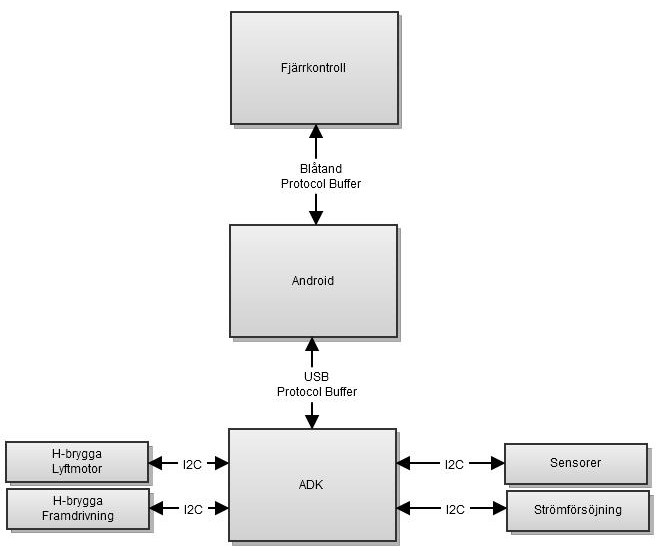
\includegraphics[width=13cm]{../includes/figures/Systemskiss} 
\caption{Systemskiss över svävaren.} 
\label{fig:Systemskiss} 
\end{figure}

Att arbeta med Android som bas för plattformar valdes för att mycket
funktionalitet fås till ett billigt pris. Ur ett
hårdvaruperspektiv så ingår det ett flertal sensorer och kommunikationskanaler
som är användbara vid utveckling av en radiostyrd enhet.

I kommande underavdelingar finns mer detaljerad information om varje delsystem.
\subsection{ADK}
Rickard\ldots
\subsection{Fjärrkontroll}
Som nämnt i avsnitt \ref{subsec:system/fjarrkontroll} så har Fjärrkontrollen tre
stora uppgifter: generera styrsignaler till svävaren, kommunicera med de andra
enheterna samt att kunna logga händelser på svävaren.

Applikationen är uppdelad tre huvudsakliga delar som var och en utgörs av en
Android-service. Dessa delar implementerar funktionalitet för kommunikation,
loggning av sensordata samt generering av styrsignaler. Applikationen innehåller
även Android-activity som fungerar som inställningsmeny för fjärrkontrollen.

Genomgång på hur kommunikationen mellan fjärrkontrollen och de andra enheterna
sker gås igenom i avsnitt \ref{subsec:commlink} och generering av
styrsignaler behandlas i \ref{subsec:styr och regler}. Nedan beskrivs hur
loggning fungerar.

\subsubsection{Loggning av sensordata}
Funktionaliteten för att logga olika typer av sensordata sker genom att kryssa
i vilka sensorer som data ska sparas i från. Insamlade data sparas som textfiler
på fjärrkontrollens SD-minne.
På den senaste versionen av applikationen finns funktionalitet för loggning av
data från fjärrkontrollens accelerometer, svävarens accelerometer samt från
svävarens ultraljudssensorer. Vilken data som skall loggas ställs in i
inställningsmenyn. Om data från svävaren önskas skickas ett kommando till den
som gör att den svarar med ett paket innehållande önskad data.

\subsubsection{Resultat}
Fjärrkontrollen möter de krav som ställs i kravspecifikationen. Vid skrivandet
av rapporten hade tester dock bara genomförts på plattformar av
smartphone-modell.

\begin {itemize}
\item Räckvidd 20 meter
\item Indikera när kommunikationen med svävaren bryts.
\item Kunna kommunicera med svävaren. Samt ge de kommandon som gränssnittet till
svävaren tillåter.
\end {itemize}

\subsubsection{Vidareutveckling}
Som brukligt så blir man aldrig riktigt klar med utveckling av mjukvara, det
finns alltid saker att finslipa. Loggningsfunktionen bör kontrolleras noggrant
och utökas så att fler sensorer går att logga. Protocol Buffer är inte
implementerat som protokoll och det skulle med relativ enkelhet kunna ändras.

\subsection{Router}
Routerns uppgifter är att handha reglersystemet och att agera som
kommunikationslänk mellan de olika enheterna.

Programmet är indelat i tre Android-services och en Android-activity:
\begin{itemize}
	\item Bluetoothservice som hanterar all Bluetoothkommunkation,
	\item UsbService som hanterar all USBkommunkation,
	\item ControlSystemService som implementerar reglersystemet
	\item och MainActivity som implementerar användargränssnittet.
\end{itemize}

Applikationen startas automatiskt genom att ansluta ADK:n till router-telefonen. 
Om applikationen körs innan den ansluts till ADK:n kommer den att startas om för
att upprätta USB-kommunikationen.
När appen körs visas en diod för respektive kommunkationsbuss. Om kommunkationen
fungerar lyser dioden grönt och om den inte fungerar så lyser den rött. Dioden
kan även lysa gult men detta är inget man hinner se i vanliga fall då den enbart
gör så under uppkoppling. Knappen "Bluetooth setup" används för att upprätta en
Bluetoothlänk.

Intern kommunkation inom applikationen sker via Android Broadcasts.
Kommunikationen med andra enheter behandlas i avsnitt \ref{subsec:commlink} och
reglersystemet behandlas i \ref{subsec:styr och regler}.

\subsubsection{Resultat}
Programmet är stabilt och uppfyller alla krav. Dess huvudsyfte är att ta emot
och skicka vidare meddelanden vilket fungerar utmärkt.
\subsection{H-brygga}
\ldots
\subsection{Motorer och fläktar}
De lyftfläktar som används är fyra stycken centrifugalfläktar som generellt sett
inte ger lika mycket luftflöde som axiella fläktar men ger däremot mycket högre
lufttryck istället. Genom att placera de fyra fläktarna parallellt med varandra
blir luftflödet ungefär fyra gånger större än för en fläkt och ger därmed ett
tillräckligt luftflöde. Ett högt lufttryck ger bidrag till att svävaren kan bära
en större totalvikt. Se specifikation av centrifugalfläkten i Tabell
\ref{tbl:fan_spec} och se mer information i datablad \cite{Delta_BFB1212VH-R00}
. Mer information kring hur lyftkraftsberäkningarna gjordes fås i Appendix
\ref{app:lyftkraftsberakningar}.

\begin{table}[htbp!]
\centering
\caption{Specifikation av centrifugalfläkt.}
\label{tbl:fan_spec}
\begin{tabular}{|l|r|}
\hline
Märkspänning & 12 V\\
\hline
Driftspänning & 4,0 - 13,8 V\\
\hline
Ström & 1,25 A\\
\hline
Effekt & 15,00 W\\
\hline
Rotationshastighet & 3100 rpm\\
\hline
Maximalt luftflöde & 1,120 m$^3$/min\\
\hline
Maximalt lufttryck & 323,6 Pa (33,00 mmH$_2$O)\\
\hline
Ljudnivå & 56,5 dB-A\\
\hline
\end{tabular}
\end{table}

Till drivningen används två stycken elmotorer (DC) som driver varsin propeller.
Se specifikation av motorn i Tabell \ref{tbl:motor_spec} och se mer information
i datablad, \cite{Motraxx_XFLY400-12}.

\begin{table}[htbp!]
\centering
\caption{Specifikation av elmotor.}
\label{tbl:motor_spec}
\begin{tabular}{|l|r|}
\hline
Märkspänning & 12 V\\
\hline
Driftspänning & 6 - 15 V\\
\hline
Tomgångsvarvtal & 21000 rpm\\
\hline
Tomgångsström & 0,6 A\\
\hline
Maximal effekt & 42,1 W\\
\hline
VID MAXIMAL EFFEKTIVITET &\\
\hline
Lastvarvtal & 19000 rpm\\
\hline
Strömförbrukning & 2,5 A\\
\hline
Vridmoment & 1,00 Nmm\\
\hline
Avgiven effekt & 19,5 W\\
\hline
Effektivitet (verkningsgrad) & 65\%\\
\hline
\end{tabular}	
\end{table}

\subsection{Strömförsörjning}
Strömförsörjningen designades med moduläritet i  åtanke så att flera olika
spänningsnivåer uppnås genom samma design på kretskort. De olika
strömförsörjningskorten som det designades för är:
\begin{itemize}
	\item 3,3 V, 3 A, med en felmarginal på $\pm$0.2 V.
	\item 5 V, 3 A, med en felmarginal på $\pm$0.5 V.
	\item 12 V, 3 A, med en felmarginal på $\pm$0.8 V.
	\item En justerbar spänningsnivå med en felmarginal på $\pm$10 \% av den
önskade spänningen och kunna leverera 3 A.
\end{itemize}

Varje typ av strömförsörjning skulle finnas på ett separat PCB, dock med samma
layout för enkel tillverkning och att eventuell beställning av kort skulle vara
billig.

Strömförsörjningarna designades också så att de gick att parallellkoppla, både
på ingångs- och utgångssidan. Detta för att kunna utöka kapaciteten vid behov.

För att uppnå kraven och för att nå god effektivitet så används switchade
regulatorer, för mer teori och val av design och komponenter se Appendix
\ref{apx:PSU}.

\subsubsection{Resultat}

Totalt 6 stycken strömförsörjningskort används i svävaren och versionerna som
konstruerades är:
\begin{itemize}
\item 2 stycken justerbara 13.8 V som driver lyftfläktarna (ett
strömförsörjningskort till två fläktar).
\item 2 stycken justerbara 10 V för drivning av drivfläktarna (ett
strömförsörjningskort per fläkt).
\item 1 stycke 12 V till drivkretsarna på båda H-bryggorna.
\item 1 stycke 5 V för ADK och logikkretsarna på båda H-bryggorna.
\end{itemize}

Korten klarar av att hålla både ström och spänningsnivåerna bra utan störningar
eller spikar.

\subsubsection{Diskussion}
Då kraven på strömförsörjningen specificerades så var det inte bestämt om det
skulle byggas ett nytt chassi med andra motorer eller inte. Därför så valdes
spännings och strömnivåer från den gamla svävaren som grund och korten
designades därefter. Detta ledde till att det behövdes fler
strömförsörjningskort än planerat. Men det medförde dock inte några problem och
detta tack vare det modulära tänkandet.

Vid för tung belastning, t.ex med starkare motorer och fläktar,
sjunker spänningen och strömmen ökar och därav bör det användas säkringar
på 4-6~A.

Det visade sig att de justerbara spänningsnivå korten var ett mycket bra val, då
vi lätt kunde öka nivån för fläktar och motorer så bäst funktion kunde erhållas.
Vid de högre spänningarna är det värt att notera att det behövdes kylflänsar
på regulatorerna.

Strömförsörjnningskorten har plats för filterkomponenter både innan regulatorn
och efter, dessa platser är i nuläget tomma och förbikopplade då inga större
störningar eller spikar kunnat uppmätas.

\subsubsection{Förbättringar}
I själva designen för strömförsörjningskorten så bör man inkludera en en
diod som förhindrar backspänning från de andra korten som lägger sig
över avstängda kort. Problemet kan återskapas lätt genom att stänga av ett
strömförsörjningskort men att ha det sammankopplat med andra
strömförsörjningskort som är i drift. Då kan statusdioder lysa trots att kortet
är avstängt. Den backspänning som uppkommer gör ingen skada på
strömförsörjningskorten, men det är lite förvillande att ett korts statusdioder
lyser trots att kortet är avstängt. Notera även  att det är H-bryggorna som
bidrar med att denna backspänning uppstår då de har flera spänningar inkopplade.

Då nuvarande strömförsörjning inte klarar att ge mer än 3 A vid sin
spänningsnivå begränsar det, mer än förväntat, val av motorer och fläktar. Så
ett strömförsörjningskort designat för högre ström skulle vara en klar
förbättring. Detta skulle också minska antalet strömförsörjningskort.
För detta kort rekommenderas det att man ej använder en färdig regulator utan
själv bygger upp det för att få bra funktion och strömbegrännsning.

\newpage
\subsubsection{Ekonomi}
Kostnad för komponenterna för de olika spänningsnivåerna ses i tabellerna \ref{gemensammadelar} - \ref{justerbar}.

\begin{table}[htbp]
\centering
\caption{Gemensamma delar}
\begin{tabular}{|l|l|r|r|}
\hline
\textbf{Komponent} & \textbf{Information} & \textbf{Antal} & \textbf{Pris} \\ 
\hline
Kondensator & 680uF, 35V & 1 & 5,68 \\ 
\hline
Schottky diod & SB540 & 1 & 6,05 \\ 
\hline
Tryckvippströmställare & R19U-R112A-B-2-B-M2 & 1 & 9,03 \\ 
\hline
Molex hane & 2p & 2 & 4,56 \\ 
\hline
Stiftdon 90\degree & 2p & 2 & 9,86 \\ 
\hline
Säkringshållare & 6,3A & 2 & 3,07 \\ 
\hline
Lysdiod & 1224-10SYGC/S530-E2 & 2 & 1,49 \\ 
\hline
\textbf{Total} &  & \multicolumn{1}{l|}{} & 39,74 \\ \hline
\end{tabular}
\label{gemensammadelar}
\end{table}


\begin{table}[htbp]
\centering
\caption{5~V Strömförsörjning}
\begin{tabular}{|l|l|r|r|}
\hline
\textbf{Komponent} & \textbf{Information} & \textbf{Antal} & \textbf{Pris} \\
\hline
Switch regulator, 5V, TO-220  & LM2596T33 & 1 & 52,62 \\ 
\hline
Spole &  47 UH  & 1 & 16,73 \\ 
\hline
Kondensator & 330UF, 35V & 1 & 5,86 \\ 
\hline
\textbf{Total} &  & \multicolumn{1}{l|}{} & 114,95 \\ 
\hline
\end{tabular}
\label{5vstrom}
\end{table}


\begin{table}[htbp]
\centering
\caption{12~V Strömförsörjning}
\begin{tabular}{|l|l|r|r|}
\hline
\textbf{Komponent} & \textbf{Information} & \textbf{Antal} & \textbf{Pris}  \\ 
\hline
Switch regulator, 12V, TO-220  & LM2596T-12  & 1 & 59,58 \\ 
\hline
Spole & 47 uH  & 1 & 16,73 \\ 
\hline
Kondensator & 180UF, 35V & 1 & 2,33 \\ 
\hline
\textbf{Total} &  & \multicolumn{1}{l|}{} & 118,38 \\ 
\hline
\end{tabular}
\label{12vstrom}
\end{table}


\begin{table}[htbp!]
\centering
\caption{Justerbar spänning strömförsörjning}
\begin{tabular}{|l|l|r|r|}
\hline
\textbf{Komponent} & \textbf{Information} & \textbf{Antal} & \textbf{Pris} \\
\hline
Switch regulator, justerbar, TO-220  & LM2596T-ADJ  & 1 & 56,73 \\ 
\hline
Spole  & 68uH & 1 & 16,73 \\ 
\hline
Kondensator & 220UF, 35V  & 1 & 3,91 \\ 
\hline
\textbf{Total} &  & \multicolumn{1}{l|}{} & 117,11 \\ 
\hline
\end{tabular}
\label{justerbar}
\end{table}

Även dessa kort beställdes från ITead Studio för en kostnad av 369,50 SEK, vilket ger en sammanlagd summa av 759,68 SEK för alla strömförsörjningskort.




\subsection{Batterier}
En studie av olika batteritekniker gjordes för att se vilka som skulle klara
kraven. Valet föll på LiPo-tekniken, då denna har hög effektdensitet och är
kostnadseffektiv.

\subsubsection{Resultat}
Två stycken 5 cells LiPo-batterier på 18,5 V och 3.3 Ah används, där ett går
till enbart strömförsörjningen för lyftfläktarna (då dessa kräver högst spänning
och mest ström) och det andra till resterande elektronik. Batteriernas
specifikation kan läsas i Tabell \ref{tbl:Battery}.

\begin{table}[htbp!]
\centering
\caption{Batterispecifikation}
\label{tbl:Battery}
\begin{tabular}{l|l}
Egenskap & Värde \\
\hline
Minsta strömkapacitet & 3300 mAh\\
Konfiguration & 5S1P / 18.5V / 5Cell\\
Maximal konstant urladdning & 30C\\
Maximal toppurladdning (10 s) & 40C\\
Vikt & 480g\\
Dimensioner (l * b * h) & 139 mm * 43 mm * 35mm\\
\end{tabular}
\end{table}

Spänningsnivån på 18,5 V är framförallt på grund av att regulatorn på
strömförsörjningskortet behöver ha minst 15 V in för att kunna hålla 12 V eller
högre ut. 3.3 Ah för att klara kraven på 10 minuters drifttid vid max
påfrestning. Inget test av maximal drifttid har gjorts men tester med minst 30
minuters körning klarades.

\subsubsection{Diskussion}
Batterierna mötte kraven väl. Eventuellt så skulle man kunna minska
strömkapaciteten för att minska totalvikten på svävaren. Projektgruppen tyckte
inte att den extra kostnaden, både i tid och pengar, samt
att försämringen av prestandan var värd inköp av andra batterier.

\subsubsection{Ekonomi}
Inköpet av batterier kostade 979 SEK, inklusive tull och frakt.

\subsection{Chassi}
Vid design av chassit användes CAD-programmet SolidWorks 2012 för att göra
3D-modeller över chassits olika delar. En prototyp modellerades i SolidWorks och
tillverkades för att användas till olika tester innan det slutliga chassit
skulle designas och tillverkas.

\subsubsection{Material}
Chassit är gjort av ett lätt skivmaterial som består av två tunna “pappskivor”
med skumplast emellan. Skivorna är 3,1 mm tjocka och är lätta att klippa, skära
och limma. Skivorna skänktes till projektgruppen av Björn-Åke
Sköld för att göra en prototyp av svävaren. Materialet användes till prototypen
men även till den slutliga svävaren.

Dysorna till fläktarna är gjorda av gjutrör av papp  och träramen som håller
ihop höljet som döljer elektroniken är av furu. Till kjolen användes ett
ripstop-tyg som är ett slitstarkt tunt tyg som används bl.a. till drakar.

\subsubsection{Prototyp}
Arbetet inleddes med att göra en CAD-modell över prototypen. Den gjordes dubbelt
så stor jämfört med den svävare som en tidigare projektgrupp har byggt.
Björn-Åke trodde nämligen att man skulle kunna göra en lite större svävare men
som ändå är lättare än den gamla vid användning av hans material.

Prototypen blev 800x570 mm och 100 mm hög. Tanken var att den gamla svävaren
skulle fästas ovanpå prototypen för att se om den kunde lyfta och sväva då. En annan tanke var
att även kjolen skulle ha testats på prototypen för att sedan kunna flyttas över
till den slutliga svävaren. Eftersom det inte skulle bli helt lätt att fästa den
gamla svävaren på prototypen testades prototypen direkt med de lyftfläktar som
skulle användas. Den kunde då lyfta och hållas svävande trots att ingen kjol
användes. Kjolen designades som en variant av fingerkjol bestående av flera
segment men hann inte sys innan en idé på en ny design dök upp.

\subsubsection{Ny design}
Efter ett möte med Björn-Åke, då han fick se prototypen och CAD-modellen av
kjolen, bestämdes att både chassit och kjolen skulle konstrueras om. Detta för
att kjolsegmenten blev för små att sy och att kjolen i sin helhet inte skulle
kunna hålla kvar luften så att ett lufttryck kunde erhållas.

I den nya designen
kunde höjden halveras på svävaren och bredden ökas 3 cm, detta för att göra
sävaren stabilare. Det nya chassit har en bagkjol istället
eftersom det är lättare att sy en sådan kjol och den kan dessutom hålla kvar
luften på ett bättre sätt så ett lufttryck erhålls. En bagkjol är inte lika
flexibel som en fingerkjol när det gäller att ta sig över hinder men i detta
projekt är bagkjolen tillräckligt flexibel.

Kjolen sitter fast i en plattform med kardborreband och eftersom det försvinner
mycket luft vid kardborrefästena har inte några hål gjorts i kjolen. På så vis
erhålls även ett lufttryck i kjolen som gör att svävaren kan bära en större
totalvikt.

Plattformen som kjolen är fäst runt är 800x600 mm och består av två
plattor av det lätta skivmaterialet. Den undre plattan är lite mindre än den
övre och de sitter ihop med distanser för att få en luftspalt på 10 mm mellan
plattorna.

En träram konstruerades för att kunna fästa fläktar, motorer och elektronik
i. Den sitter fast i plattformen med kardborreband och håller även ihop höljet
som döljer elektroniken med kardborreband.

Svävaren är uppbyggd på ett modulärt sätt och de olika delarna är placerade på
ett sätt som ger låg tyngdpunkt. Den är även uppbyggd symmetriskt med en jämn
viktfördelning över hela svävarens bottenyta. En 3D-modell över svävaren visas i
Figur \ref{fig:CAD_Hover}.

\begin{figure}[htbp!] 
\centering 
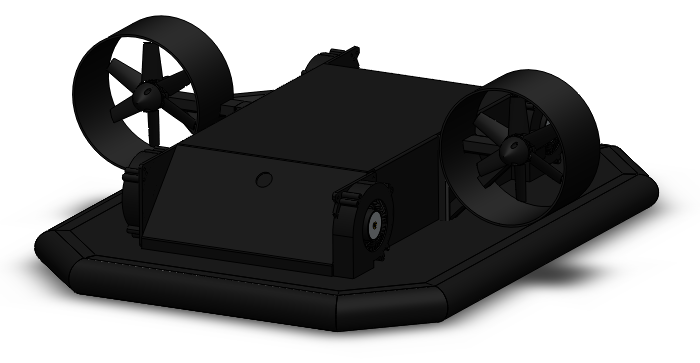
\includegraphics[width=8cm]{../includes/figures/CAD_Hovercraft.png} 
\caption{3D-modell över svävaren.} 
\label{fig:CAD_Hover} 
\end{figure}

\subsubsection{Vidareutveckling}
I en vidareutveckling av svävaren skulle materialet kunna bytas ut mot ett mer
hållbart och vattentåligt material. Skivmaterialet har en tendens att slitas
sönder när delarna ska tas isär vid kardborrefästena.

Träramen som är av furuskulle kunna bytas ut till ett lättare träslag som
balsaträ eller ett annat lätt material.

Genom att skala upp modellen kan en större svävare göras med samma design. Men
det som behöver tänkas på då är att de fläktar och motorer som väljs klarar av
den nya vikten.

\section{Funktionalitet}
Den funktionallitet som har implementerats i mjukvaran har delats upp i ett
antal underrubriker. Detta för att göra det tydligare för läsaren.
\subsection{Kommunikationslank}
Mjukvarugänget\ldots
\subsubsection{Protocol buffer}
Protocol Buffer\cite{Protocol buffer} är ett protokoll som används för
serialisering av data.
Protokollet är utvecklat av Google, där Google har gjort kompilatorer för Java,
C++ och Python tillgängliga. Utöver dessa kompilatorer från Google så finns det
andra kompilatorer utvecklade av privatpersoner eller företag för andra språk.

Svävaren använder sig dels av Googles javakompilator för protokollet i 
fjärrkontrollen samt telefonen. För ADK:n så används en simplare version av
Protocol Buffer nämligen Nanopb \cite{Nanopb} som implementerar protokollet i
statisk C kod.

Det Protocol Buffer generar är programkod med funktionalitet för att kunna
serialisera och deserialisera olika dataobjekt. Dessa dataobjekt beskrivs av
användaren med ett IDL (Interface Definition Language).
Svävaren använder sig av sju stycken olika dataobjekt för sin kommunikation(se
appendix xxx fil Command.proto).

\subsubsection{ADK till Telefon}
Rickard och Jens\ldots
\subsubsection{Telefon till fjärrkontroll}
Johan\ldots

\subsection{Styr- och reglersystem}
\label{subsec:styr och regler}
För att styra svävaren samlas acclerometerdata in i realtid på fjärrkontrollen som sedan processeras och omvandlas till styrsignaler som skickas till routern där det även finns plats för ett reglersystem.

\subsubsection{Styrsystem}
Det finns tre olika styralgorithmer för att processera pitch- och rolldata separat. De tre olika styralgorithmerna processerar acclerometerdatan på liknande sätt men med olika matamatiska funktioner, de tre lägena är logaritmisk, exponentionell och linjär. Man kan genom dropdown listor på fjärrkontrollen välja vilken styralgoritm som ska användas. De olika styralgoritmerna utvecklades med hjälp av MATLAB för att sedan implementeras i JAVA på fjärrkontrollen. De olika styralgoritmernas utslag då pitch = 30\degree  då roll går från -45\degree till 45\degree  kan ses i figur~\ref{fig:styralgoritmer}.

\begin{figure}[htbp!]
\centering
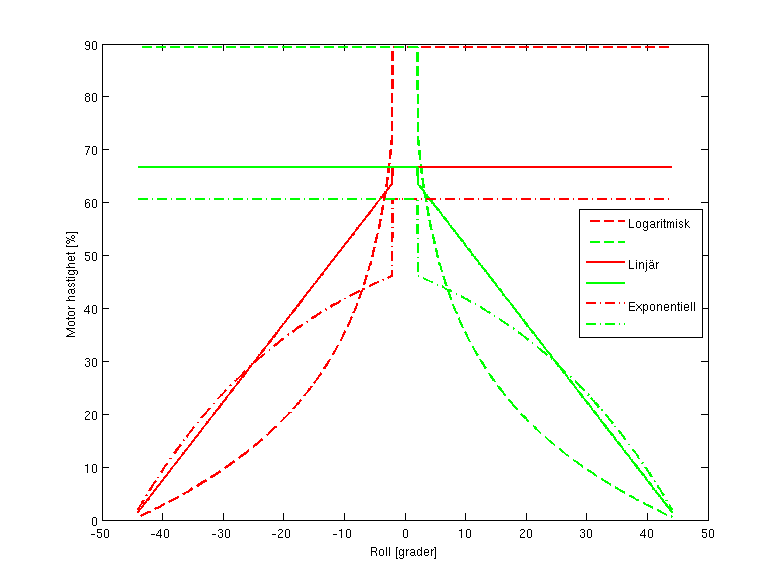
\includegraphics[width=12cm]{../../includes/figures/Styralgoritmer}
\caption{Styralgoritmernas utslag vid pitch = 30\degree då roll = [-45,45].}
\label{fig:styralgoritmer}
\end{figure}

I realiteten märkte föraren dock ingen större skillnad mellan de olika styrlägena. 

\subsubsection{Reglersystem}
Designen av svävaren medförde att hastighet och styrning var starkt korskopplade vilket medför svårigheter då en regulator ska implementeras. Grundlig efterforskning gjordes och det bestämdes att ramverket ACADO skulle användas för att implementera en regulator till svävaren då ramverket kunde autogenerera kod för mer komplexa regulatorer. Detta visade sig vara svårare än förutspått och ramverket krävde även mer minne än vad som fanns tillgängligt. Dessa bakslag medförde att reglersystemet lades på is för att kunna vidareutvecklas vid ett senare tillfälle.

\subsection{Sensorer}
Rickard och Emil\ldots
\section{Ekonomi}
Emil\ldots
\section{Användarmanual}
Följande underavdelningar beskriver hur svävaren hanteras.
\subsection{Hårdvara}

Lista för att starta svävaren:
\begin{enumerate}
\item Se till så batterierna är laddade och inkopplade.
\item Slå på de båda strömbrytarna på sidan av chassit (se till så batterierna är kopplade till dessa och att klämmorna sitter fast)
\item Slå på brytaren på alla strömförsörjningskorten (alla status dioder ska lysa stark och klart. På grund av backspänning kan dioderna lysa trots att kortet är avstängt). Brytarna på strömförsörjningskorten står med fördel påslagna hela tiden och endast chassi brytarna används.
\item Om telefon är dit kopplad så ska den nu få ström från svävaren och det är bara att koppla upp fjärrkontrollen och köra.\\
\end{enumerate}


Kort felsökning om det inte funkar:
\begin{itemize}
\item Börja kolla sladdar, sladd från batteri till chassi strömbrytaren kan lossna
\item Strömbrytare påslagna? (alla status dioder ska lysa stark och klart. På grund av backspänning kan dioderna lysa trots att kortet är avstängt)
\item Får inte telefonen kontakt med adk? Lyser dioder på Adk, om inte se till så att 5 V kontakt är ansluten till Adk och strömförsörjning påslagen. Om påslaget och dioder lyser testa att  trycka på reset knappen på Adk. Fortfarande inget? Dra ur usb kontakt till telefon. 
\item Går lyftfläktarna ojämnt? Kolla spännings nivå ut från de strömförsörjningskkort till fläktarna och se så de är lika annars skriva lite på potentiometern för att ändra.
\item Går inte framdrivningsfläktarna? Kolla så alla strömförsörjningskort är påslagna, H-bryggorna behöver 5 V, 12 V och en justerbar spänning för drivning av fläktarna.
\end{itemize}

\subsection{Sammankoppling av telefoner}

När telefonen på svävaren är inkopplad till ADK:n och dess applikation har startat kan
bluetoothlänken till fjärrkontrollen upprättas. För att upprätta denna länk finns det några steg som skall göras på de olika sidorna, dessa steg beskrivs nedan.

\subsubsection{Svävaren}

För att initiera länken trycker man på knappen Bluetooth Setup i applikationen på svävaren.
När denna knapp har trycks så har man 30 sekunder på sig att ansluta till den med fjärrkontrollen, om man inte ansluter inom den tiden så kopplas länken ner igen.
Telefonens på svävaren måste vara synlig för andra bluetoothenheter för att den skall kunna upptäckas av fjärrkontrollen.

\begin{figure}[htbp!]
\centering
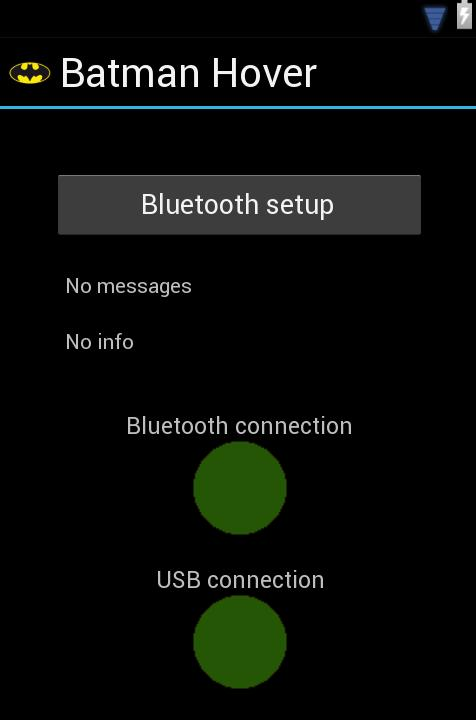
\includegraphics[width=4cm]{../../includes/figures/hoverApp.png}
\caption{Grafiskt interface för applikationen på svävaren.}
\label{fig:hoverApp}
\end{figure}


\subsubsection{Fjärrkontrollen}

På fjärrkontrollen finns det tre knappar som används vid sammankopplingen, dessa är Search, Choose samt Connect. Med Search-knappen leter fjärrkontrollen efter tillgängliga bluetoothenheter i dess omgivning. När denna sökning är klar så listas alla upptäckta enheter i applikationen under Inforubriken. Med knappen Choose kan man stega genom listan med upptäckta enheter tills man kommer fram till den man vill ansluta sig till, alltså svävaren.
Search och Choose kan göras innan knappen Bluetooth Setup har tryckts i applikationen på svävaren. När man med Choose har valt svävaren på fjärrkontrollen och Bluetooth Setup har trycks på applikationen på svävaren trycks slutligen knappen Connect på fjärrkontrollen, då sammankopplas telefonerna och länken för dataöverföring är öppen.

\begin{figure}[htbp!]
\centering
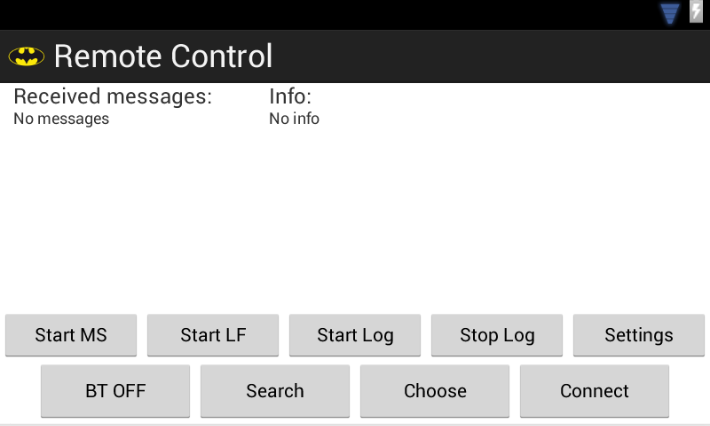
\includegraphics[width=8cm]{../../includes/figures/remoteApp.png}
\caption{Grafiskt interface för applikationen på fjärrkontrollen.}
\label{fig:remoteApp}
\end{figure}

\subsection{Styrning av svävare}
\ldots
\subsection{Loggning av data}
\ldots
\section{Slutord}
\ldots
\begin{thebibliography}{9}
\bibitem{Motraxx_XFLY400-12}{}
Motraxx,
\emph{Motraxx XFLY400-12}. \\
\url{http://files.voelkner.de/225000-249999/238829-da-01-ml-Elektromotor_XFLY400
_12_de_en.pdf},
\\ hämtad 2013-01-13.
\bibitem{Delta_BFB1212VH-R00}{}
Delta,
\emph{BFB1212VH-R00 (BFB120x120x32mm)},\\
\url{http://www.delta.com.tw/product/cp/dcfans/download/pdf/BFB/
BFB120x120x32mm.pdf},
\\ hämtad 2013-01-13.

\bibitem{Protocol buffer}{}
Google,
\emph{Protocol Buffers – Google's data interchange format – Google Project
Hosting}, \\
\url{http://code.google.com/p/protobuf/} \\
hämtad 2012-12-10.

\bibitem{Nanopb}{}
Petteri Aimonen,
\emph{Nanopb - protocol buffers with small code size}, \\
\url{http://koti.kapsi.fi/jpa/nanopb/} \\
hämtad 2012-12-10.

\bibitem{Source code}{}
Daniel Josefsson et al.,
\emph{Källkod för svävare}, \\
\url{https://github.com/jenmo917/TNE085} \\
hämtad 2012-01-15.

\bibitem{AOAA}{}
Embedded Artists,
\emph{Android Open Accessory Application Kit}, \\
\url{http://www.embeddedartists.com/products/app/aoa_kit.php} \\
hämtad 2012-01-14.

\bibitem{Arduino ADK}{}
Arduino,
\emph{ADK}, \\
\url{http://arduino.cc/en/Main/ArduinoBoardADK} \\
hämtad 2012-01-14.

\bibitem{Eclipse_ArduinoCore}{}
Arduino,
\emph{Arduino för Eclipse}, \\
\url{http://playground.arduino.cc/code/eclipse} \\
hämtad 2012-01-15.

\bibitem{USBHost}{}
Arduino,
\emph{USB\_Host Library}, \\
\url{http://labs.arduino.cc/ADK/AccessoryMode} \\
hämtad 2012-01-14.

\bibitem{Wire}{}
Arduino,
\emph{Wire Library}, \\
\url{http://arduino.cc/en/Reference/Wire} \\
hämtad 2012-01-14.

\bibitem{Eventsystem}{}
mromani, Arduino forum user,
\emph{Event System}, \\
\url{http://arduino.cc/forum/index.php/topic,37650.0.html} \\
hämtad 2012-01-14.

\bibitem{kompass}{}
Sparkfun,
\emph{Kompassmodul}, \\
\url{https://www.sparkfun.com/products/7915} \\
hämtad 2012-01-14.

\bibitem{ITead Studio}{}
ITead Studio,
\emph{PCB Manufactor}, \\
\url{http://imall.iteadstudio.com} \\
hämtad 2012-01-15.
\end{thebibliography}


\appendix
\section{Lyftkraftsberäkningar}
Teoretiska beräkningar utifrån prestandan av centrifugalfläktarna. Hur stort
luftflödet är från fläktarna och hur högt lufttryck de klarar av att hålla är
två viktiga aspekter att ta hänsyn till vid implementation i svävaren.

\subsection{Luftflöde och lufttryck}
Luftflöde och lufttryck för fläktarna fås ur datablad,
\cite{Delta_BFB1212VH-R00}, där lufttrycket har räknats om till Pascal. Då de
fyra fläktarna placeras parallellt med varandra antas lufttrycket vara det samma
som för en fläkt medan det totala luftflödet får bidrag från varje fläkt och
multipliceras därmed med fyra. \\ \\
Luftflöde: $1,12\ m^3/min$ per fläkt \\
\begin{math}
\Rightarrow 4\times1,12=4,48\ m^3/min
\end{math} totalt för fyra fläktar \\ \\
Lufttryck: $P_{c}=323,6\ Pa$ \\ \\
Den area som luften kan ta sig ut genom från kjolen bör inte vara större än att
luftflödet blir lika med eller mindre än luftflödet från fläktarna. För att få
en area som ger ett luftflöde lite mindre än luftflödet från fläktarna kan
totalt 40 hål göras i kjolen där varje hål har en diameter på 1cm. Det blir
alltså 9 hål på vardera långsida, 5 hål på vardera kortsida och 3 hål på vardera
hörnsida. Detta ger arean $ A_{e}$. \\ \\
\begin{math}
A_{e}=40\times\pi\times0,005^2=0,00314\ m^2
\end{math} \\ \\
Lufttrycket från fläktarna ger upphov till att luften måste tas sig ut genom
hålen i kjolen med en viss hastighet som ges av: \\ \\
\begin{math}
P_{c}=\frac{1}{2} \rho v_{e}^2\ \Rightarrow\ v_{e}=\sqrt{\frac{2P_{c}}{\rho}}
\end{math} \\ \\
där $\rho$ är luftens densitet vid havsytan i $ kg/m^3$ \\ \\
Hastigheten på luften som ska tas sig ut genom hålen i kjolen ges därmed av: \\
\\
\begin{math}
v_{e}=\sqrt{\frac{2P_{c}}{\rho}}=\sqrt{\frac{2\times323,6}{1,22}}=23,0324\ m/s
\approx 23\ m/s \end{math} \\ \\
Den volym luft (luftflöde) som försvinner ut ur hålen i kjolen ges av: \\
\begin{math}
V=A_{e}v_{e}=0,00314\times23,0324 \approx 0,0723\ m^3/s=4,3393\ m^3/min \\
\Rightarrow V \approx 4,34\ m^3/min
\end{math} \\ \\ \\
Om fästet mellan kjol och svävare skulle kunna hålla helt tätt och inga hål görs
i kjolen så att ett maximalt lufttryck skulle erhållas, då skulle fläktarna
klara av att lyfta en total vikt (svävaren+last) på ca 15 kg som ges av: \\ \\
\begin{math}
m_{tot}=\frac{P_{c}A}{g}=\frac{323,6\times0,46}{9,81}=15,17\ kg \approx 15\ kg
\end{math} \\ \\
där $A$ är svävarens bottenarea i $m^2$ \\
och $g$ är tyngdaccelerationen i $m/s^2$

\subsection{Diskussion}
Luftflödet ut ur hålen blir alltså $4,34\ m^3/min$ som är lite mindre än
luftflödet från fläktarna $(4,48\ m^3/min)$. På så vis kan ett litet lufttryck
erhållas i kjolen men med färre hål ökar lufttrycket i kjolen och svävaren kan
bära en större vikt. Eftersom kjolen fästs med kardborreband i svävaren blir det
inte helt tätt och mycket luft försvinner vid kardborrefästena. Därför har inga
hål gjorts i kjolen för att ett högre lufttryck ska kunna erhållas.

Även om fläktarna klarar av att lyfta 15 kg är det inte säkert att kjolen håller
ihop och kan därför spricka. Det skulle också bli en hög friktion mellan kjol
och golv om 15 kg skulle drivas framåt, vilket försämrar drivningen av svävaren.
En kompromiss med att använda en kjol utan hål och låta luften försvinna ut vid
kardborrefästena ger en tillräckligt låg friktion för att få en bra drivning av
svävaren. \\
% Text om slutliga svävarens vikt och lastens vikt!!
%{\color{red}Text om slutliga svävarens vikt och lastens vikt!!}

\section{Programkod}
\ldots

\section{Kretsschema \& PCB-layout}
\subsection{Kretsschema}
\begin{landscape}
\begin{figure}[htbp!]
\centering
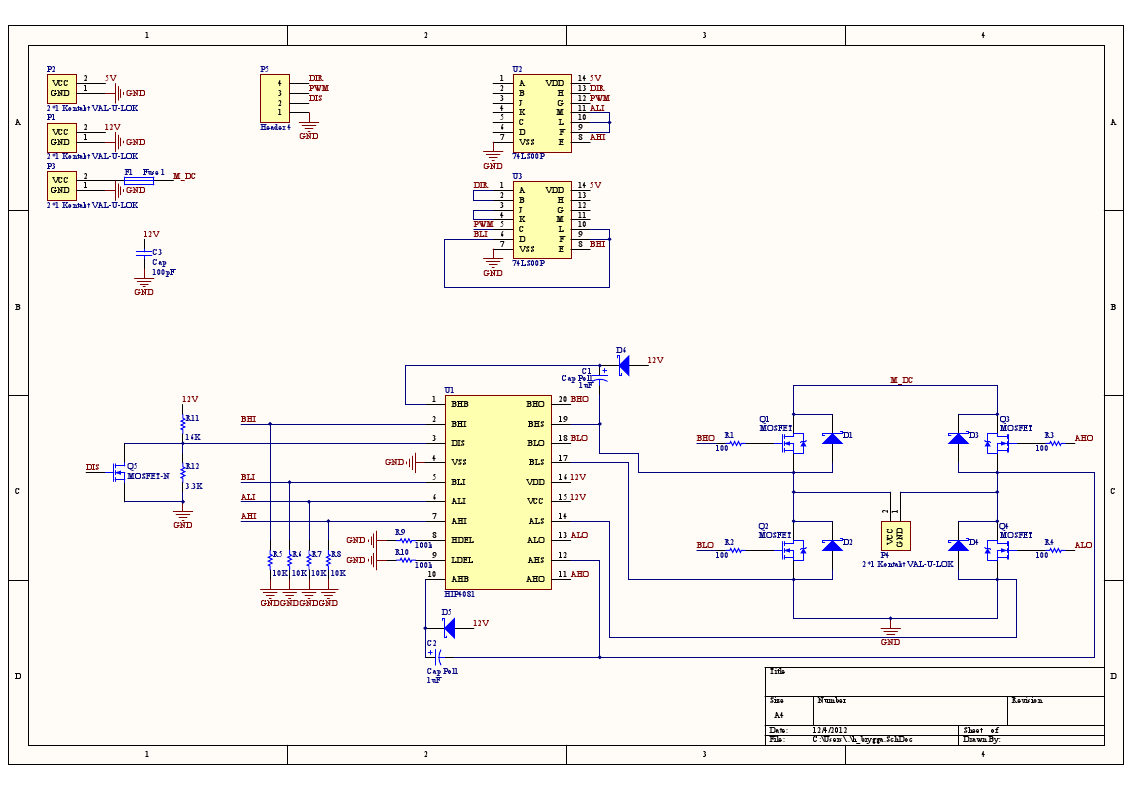
\includegraphics[width=18cm]{../../includes/figures/h_brygga_schematic}
\caption{H-bryggans kretsschema.}
\label{fig:appendix_h_brygga_schema}
\end{figure}
\end{landscape}

\begin{landscape}
\begin{figure}[htbp!]
\centering
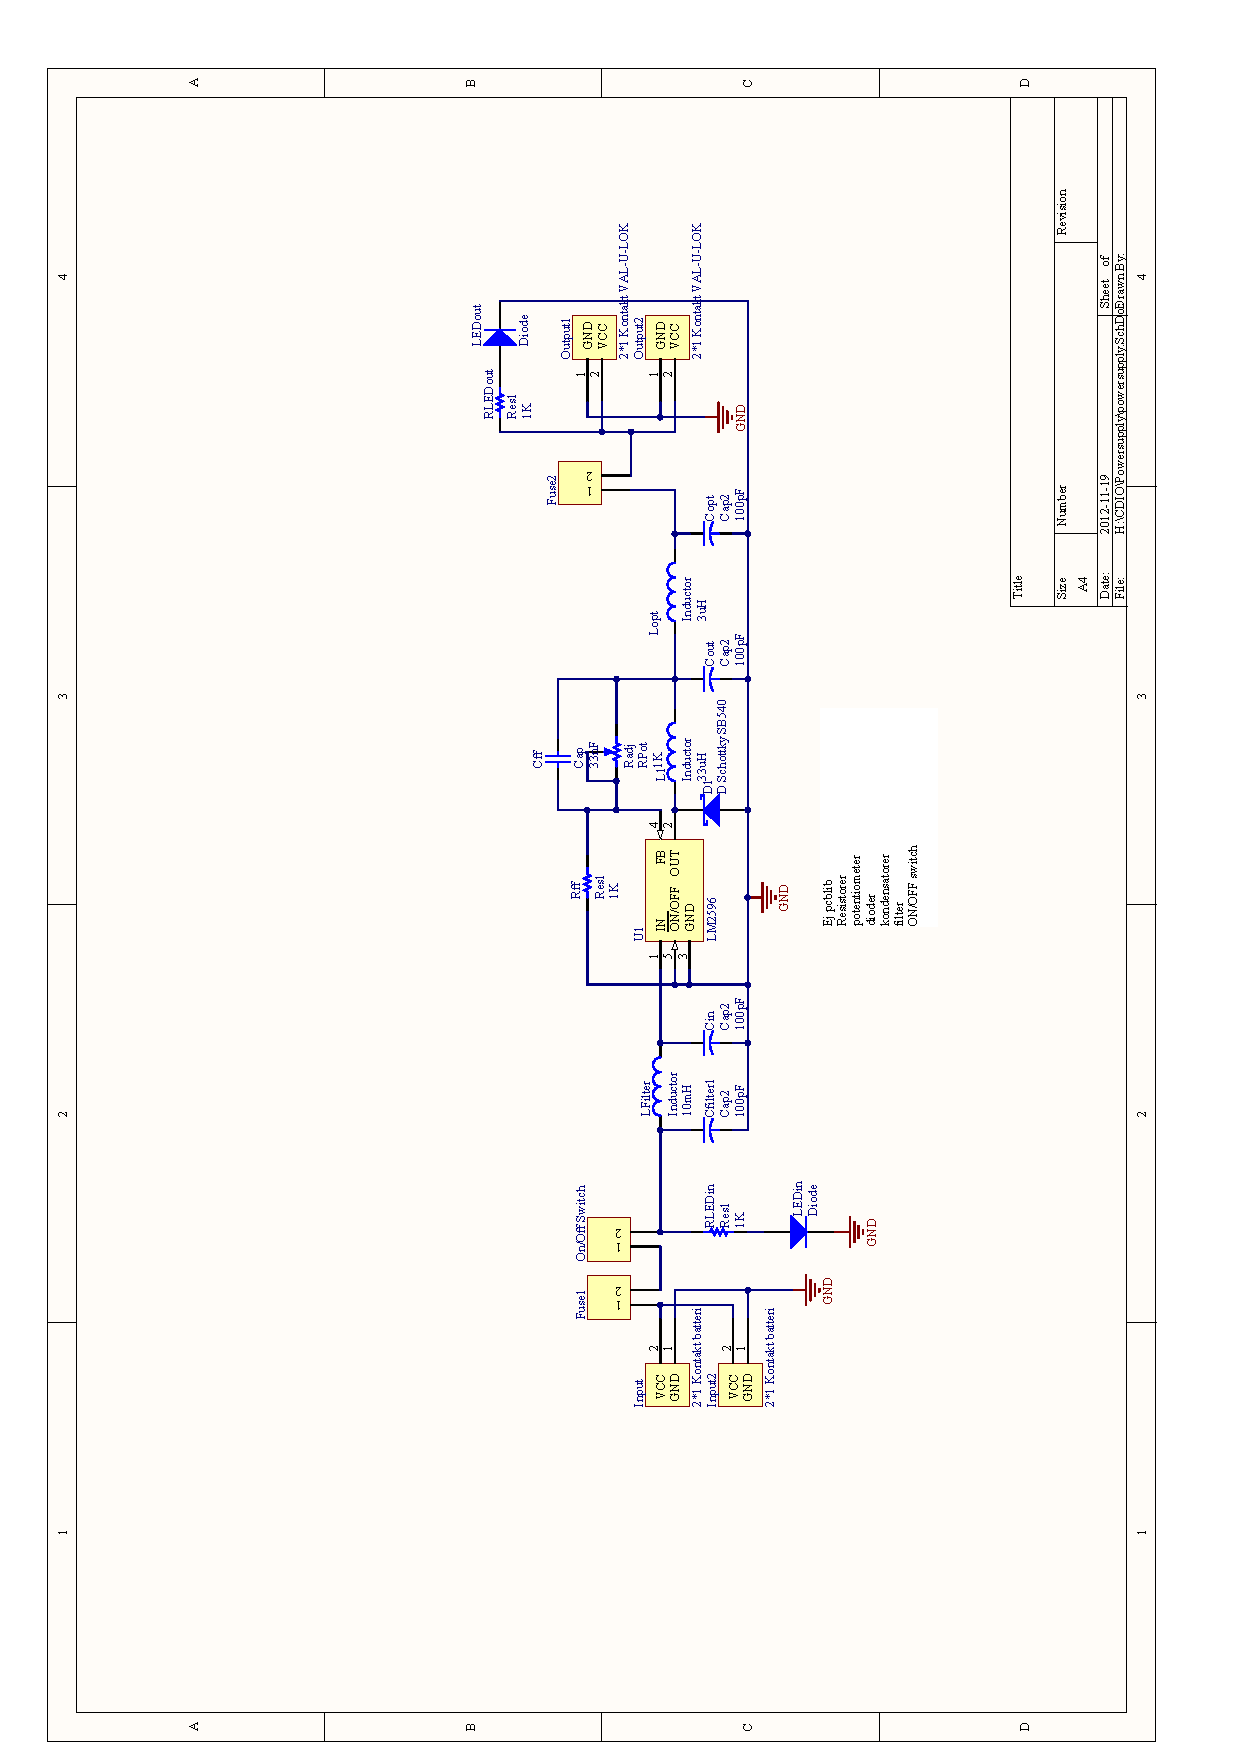
\includegraphics[height=18cm,angle=270]{../../includes/figures/PSU_Schematic}
\caption{Strömförsörjningens kretsschema.}
\label{fig:appendix_PSU_schema}
\end{figure}
\end{landscape}

\subsection{PCB-layout}
\begin{figure}[htbp!]
\centering
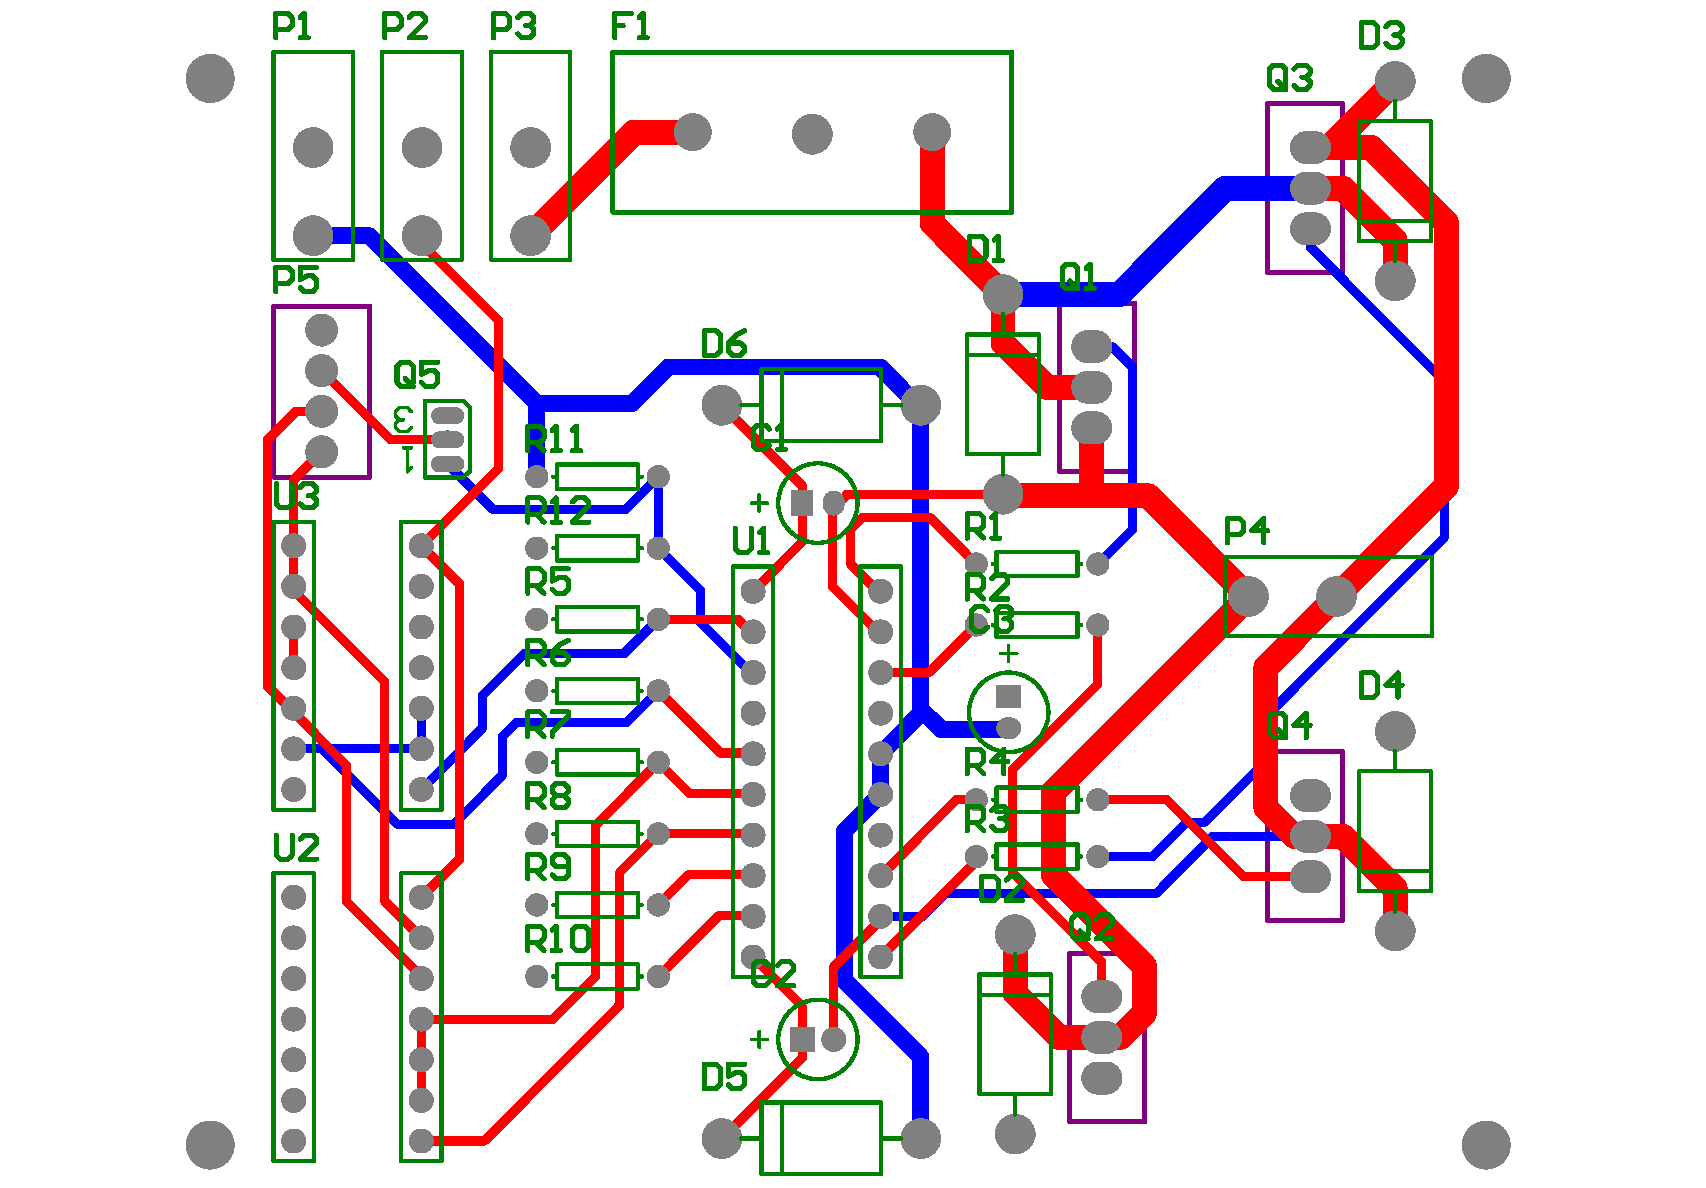
\includegraphics[width=12cm]{../../includes/figures/H_brygga_pcb}
\caption{H-bryggans PCB-layout.}
\label{fig:appendix_pcb_layout}
\end{figure}

\begin{figure}[htbp!]
\centering
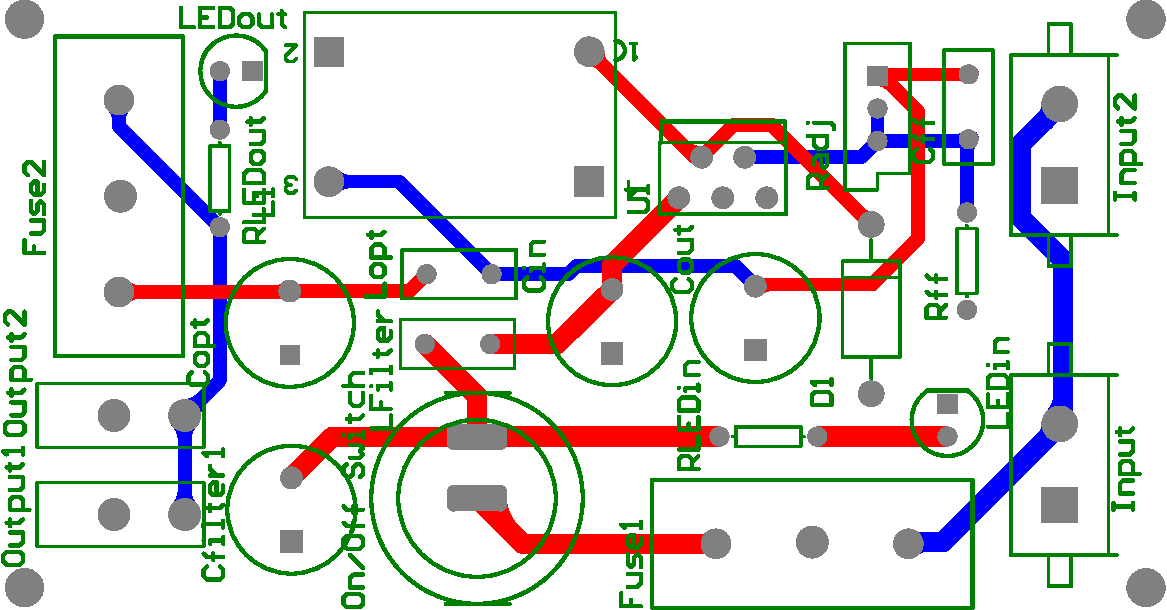
\includegraphics[width=12cm,angle=270]{../../includes/figures/PSU_PCB}
\caption{Strömförsörjningens PCB-layout.}
\label{fig:appendix_PSU_pcb_layout}
\end{figure}

\section{Chassi}
\begin{landscape}
\begin{figure}[htbp!]
\centering
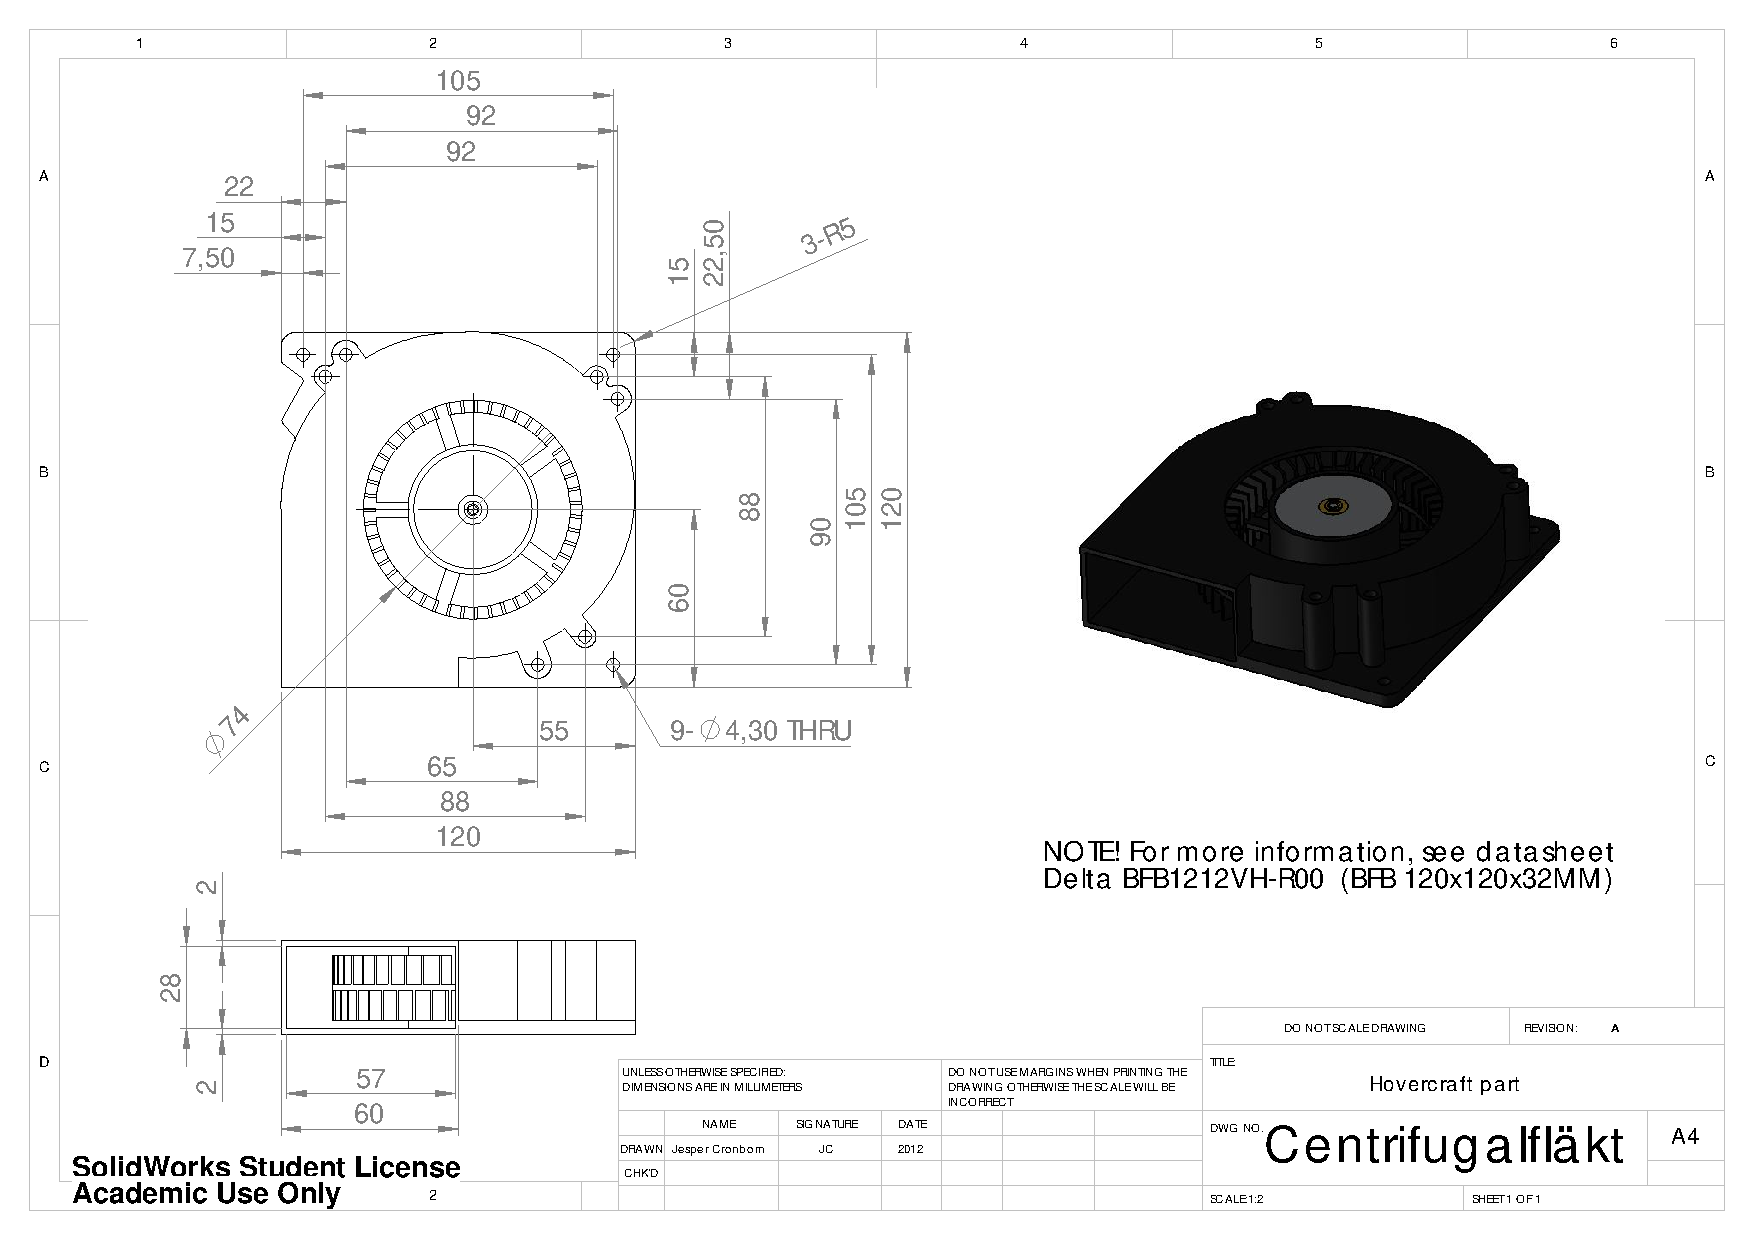
\includegraphics[width=18cm]{../../includes/figures/PDF_ritningar/Centrifugalflakt}
\caption{Ritning över centrifugalfläkt.}
\label{fig:Centrifugalfläkt}
\end{figure}
\end{landscape}

\begin{landscape}
\begin{figure}[htbp!]
\centering
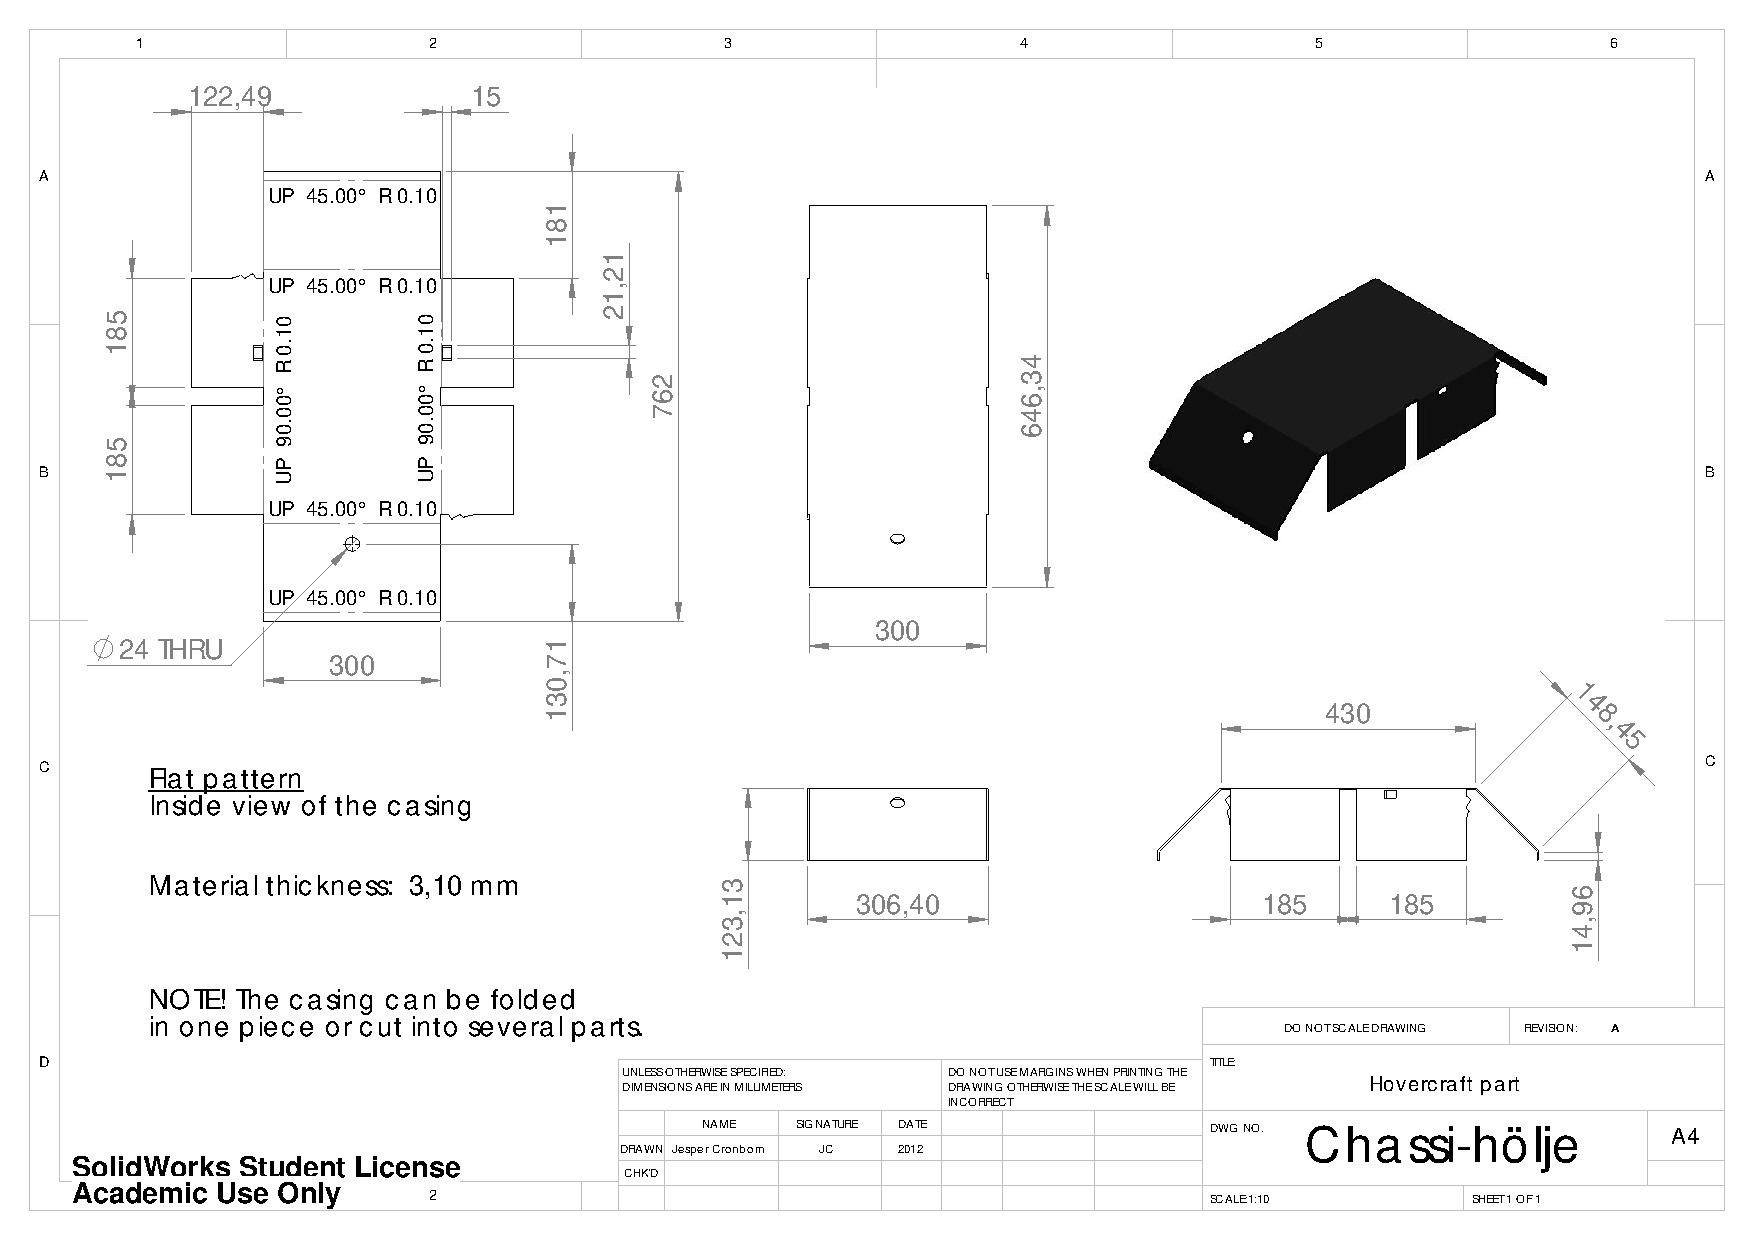
\includegraphics[width=18cm]{../../includes/figures/PDF_ritningar/Chassi_holje}
\caption{Ritning över Chassi hölje.}
\label{fig:Chassi_holje}
\end{figure}
\end{landscape}

\begin{landscape}
\begin{figure}[htbp!]
\centering
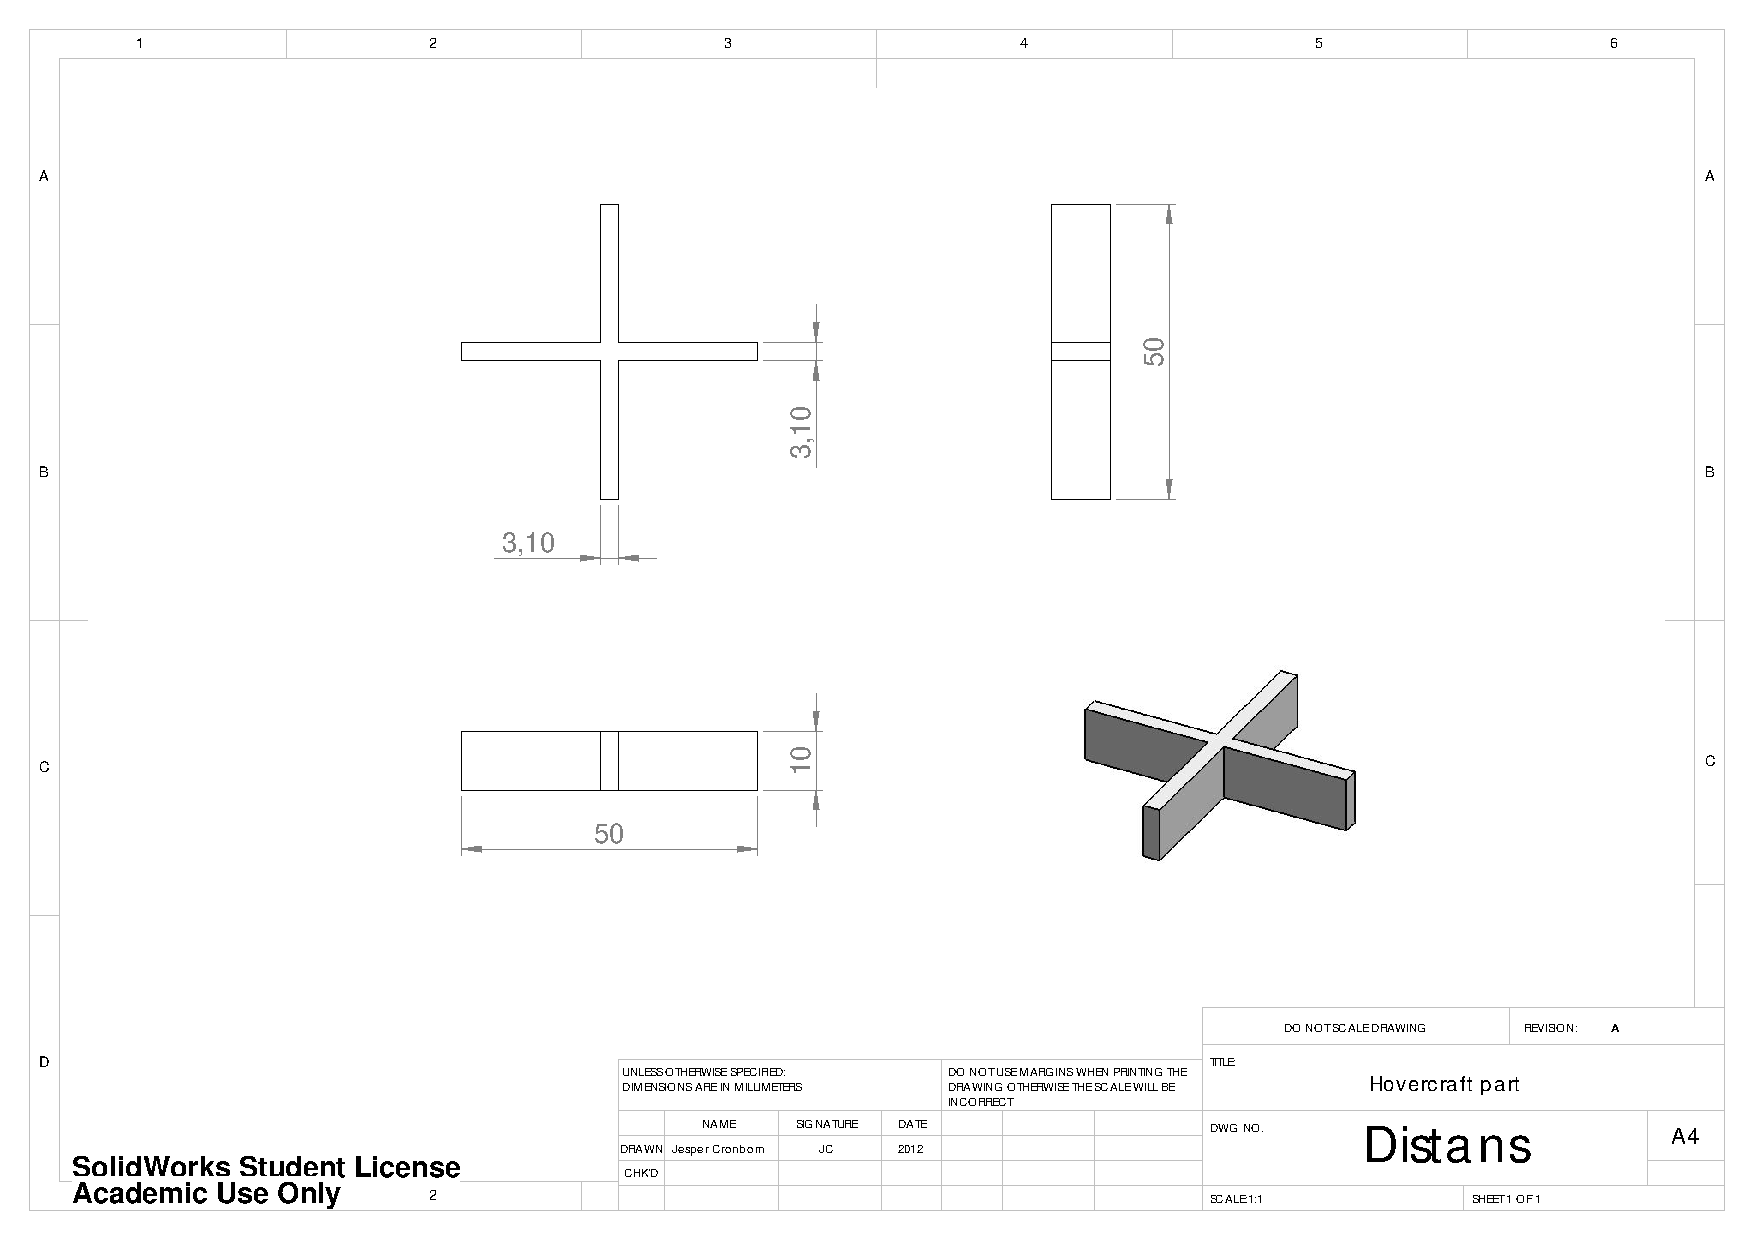
\includegraphics[width=18cm]{../../includes/figures/PDF_ritningar/Distans}
\caption{Ritning över distans.}
\label{fig:Distans}
\end{figure}
\end{landscape}

\begin{landscape}
\begin{figure}[htbp!]
\centering
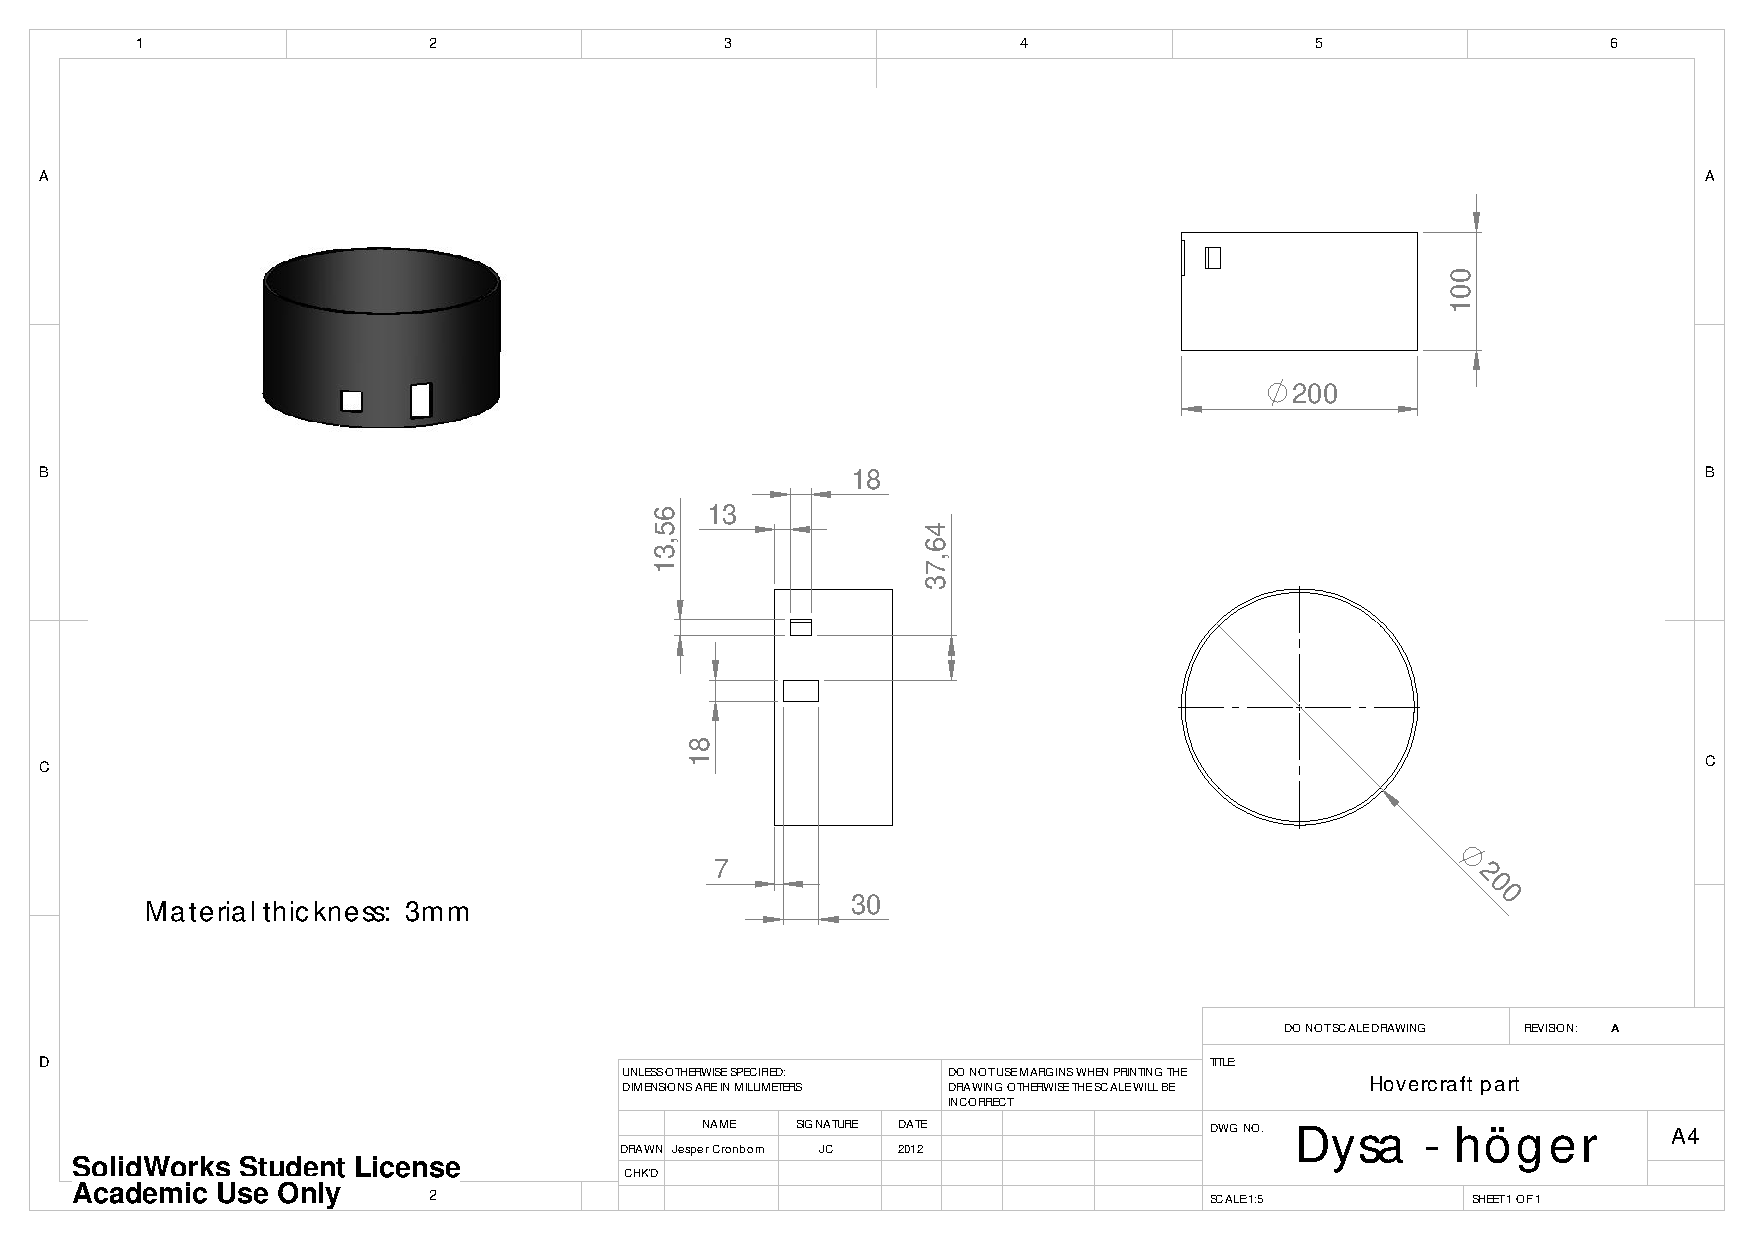
\includegraphics[width=18cm]{../../includes/figures/PDF_ritningar/Dysa_hoger}
\caption{Ritning över höger dysa.}
\label{fig:Dysa-höger}
\end{figure}
\end{landscape}

\begin{landscape}
\begin{figure}[htbp!]
\centering
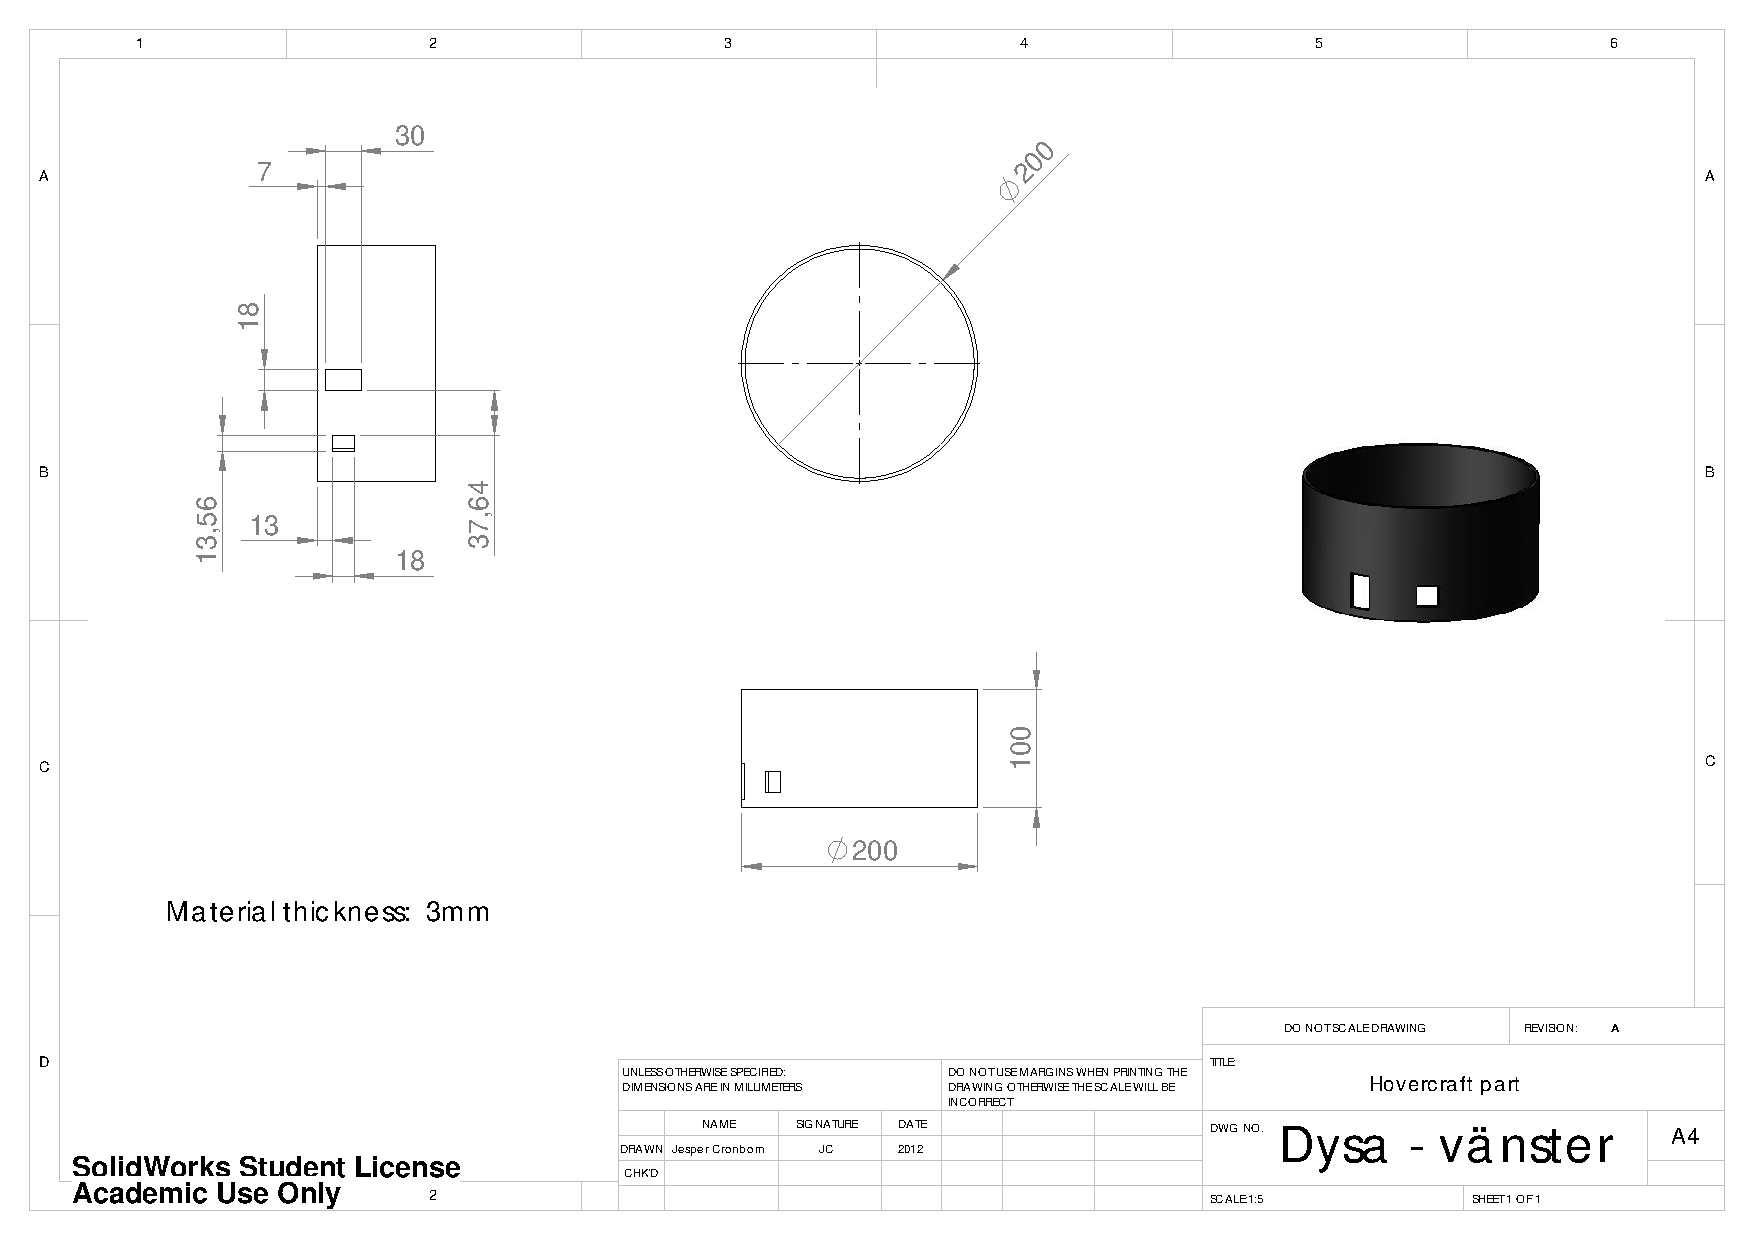
\includegraphics[width=18cm]{../../includes/figures/PDF_ritningar/Dysa_vanster}
\caption{Ritning över vänster dysa.}
\label{fig:Dysa-höger}
\end{figure}
\end{landscape}

\begin{landscape}
\begin{figure}[htbp!]
\centering
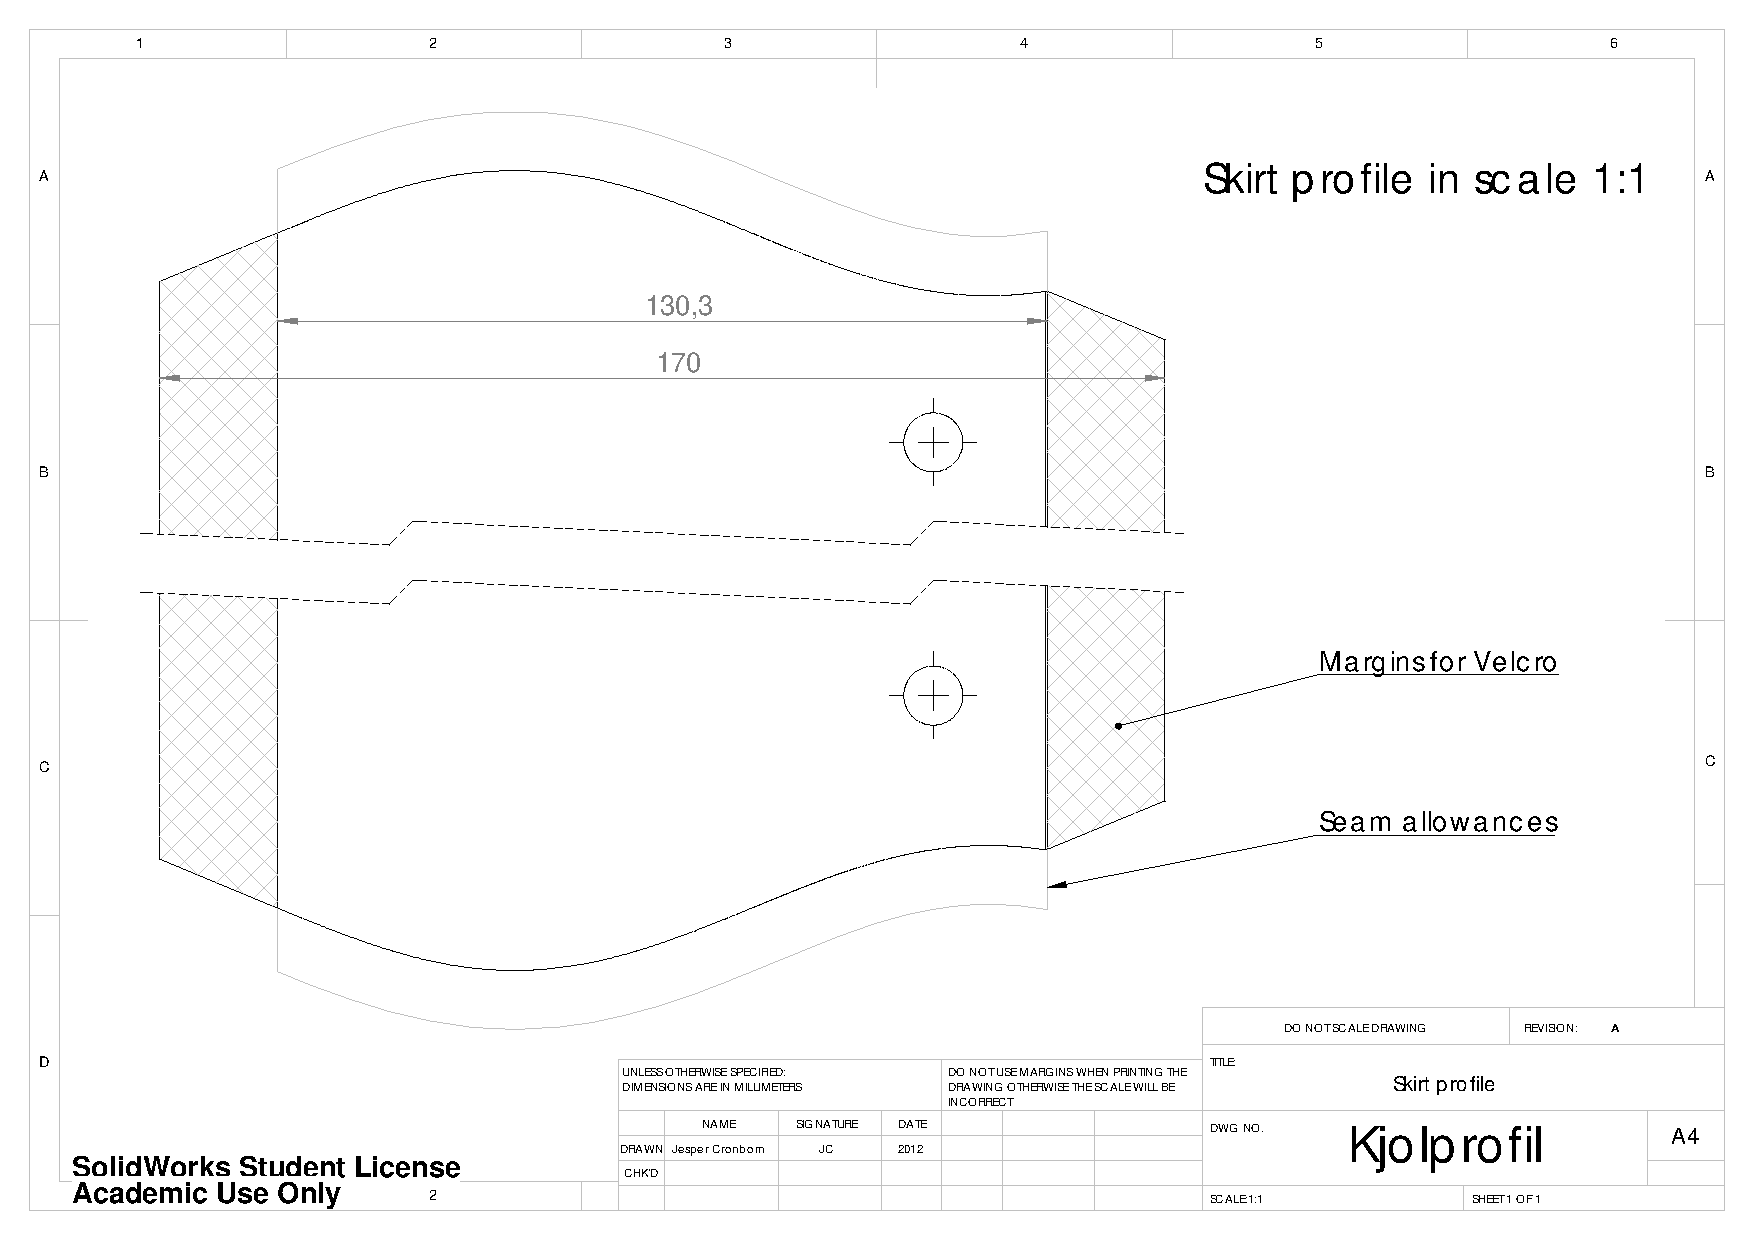
\includegraphics[width=18cm]{../../includes/figures/PDF_ritningar/Kjolprofil}
\caption{Ritning över kjolprofil.}
\label{fig:Kjolprofil}
\end{figure}
\end{landscape}

\begin{landscape}
\begin{figure}[htbp!]
\centering
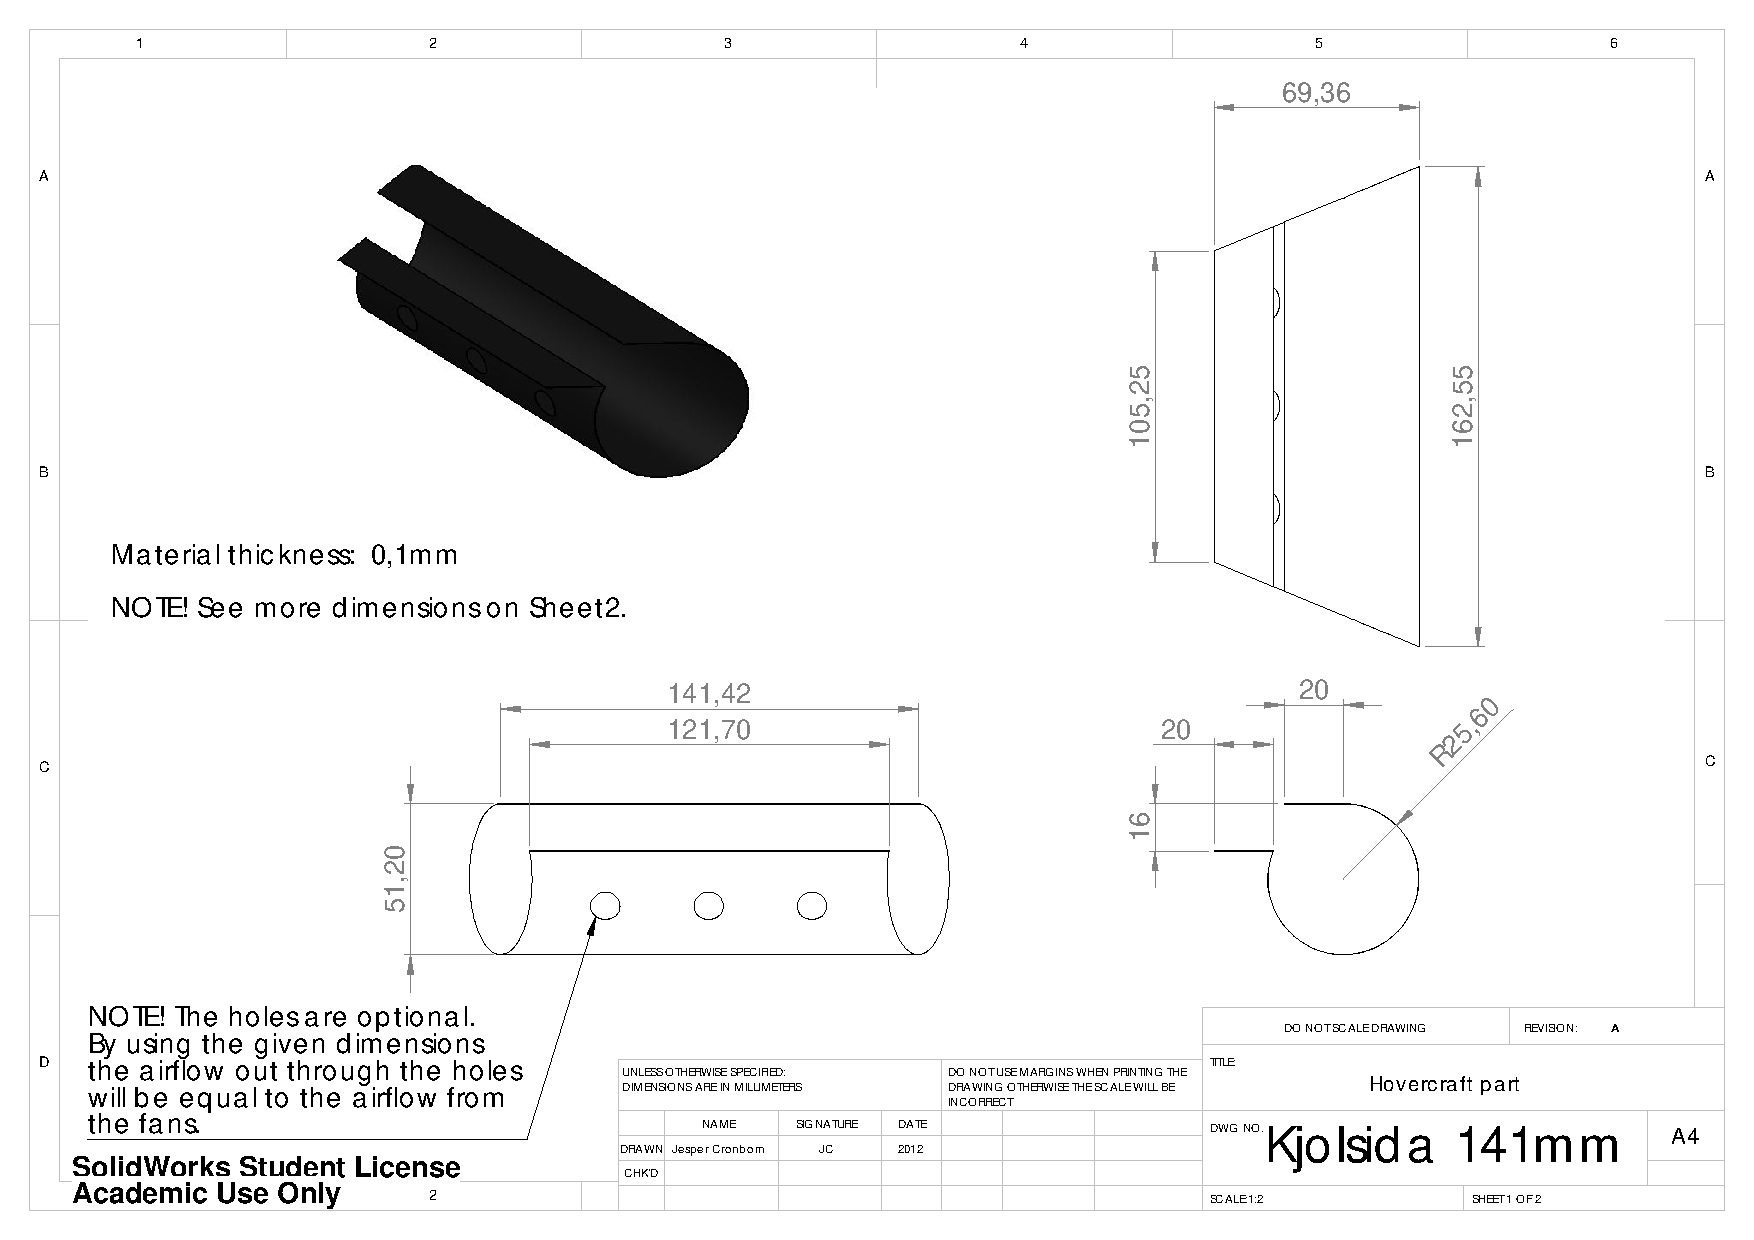
\includegraphics[width=18cm]{../../includes/figures/PDF_ritningar/Kjolsida_141}
\caption{Ritning över kjolsida 141.}
\label{fig:kjolsida141}
\end{figure}
\end{landscape}

\begin{landscape}
\begin{figure}[htbp!]
\centering
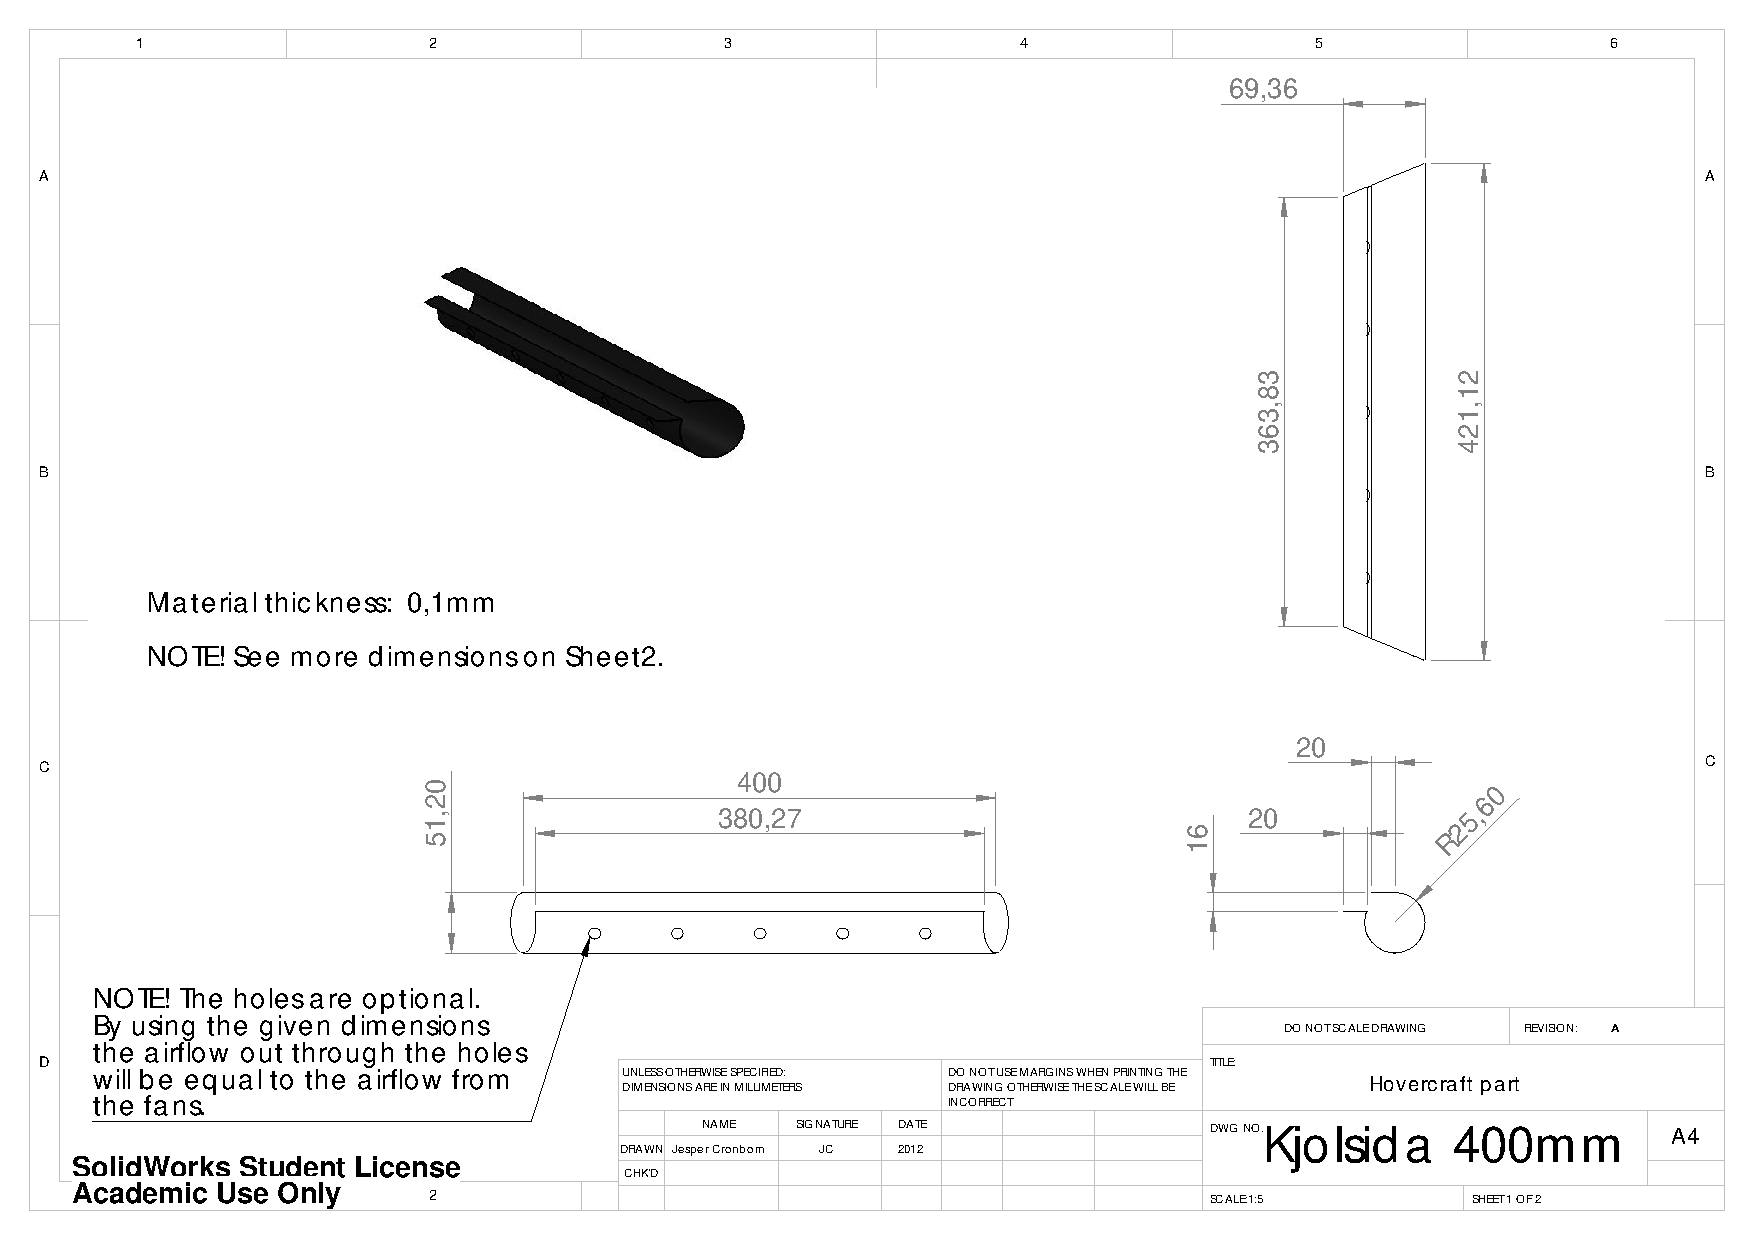
\includegraphics[width=18cm]{../../includes/figures/PDF_ritningar/Kjolsida_400}
\caption{Ritning över Kjolsida 400.}
\label{fig:Kjolsida_400}
\end{figure}
\end{landscape}

\begin{landscape}
\begin{figure}[htbp!]
\centering
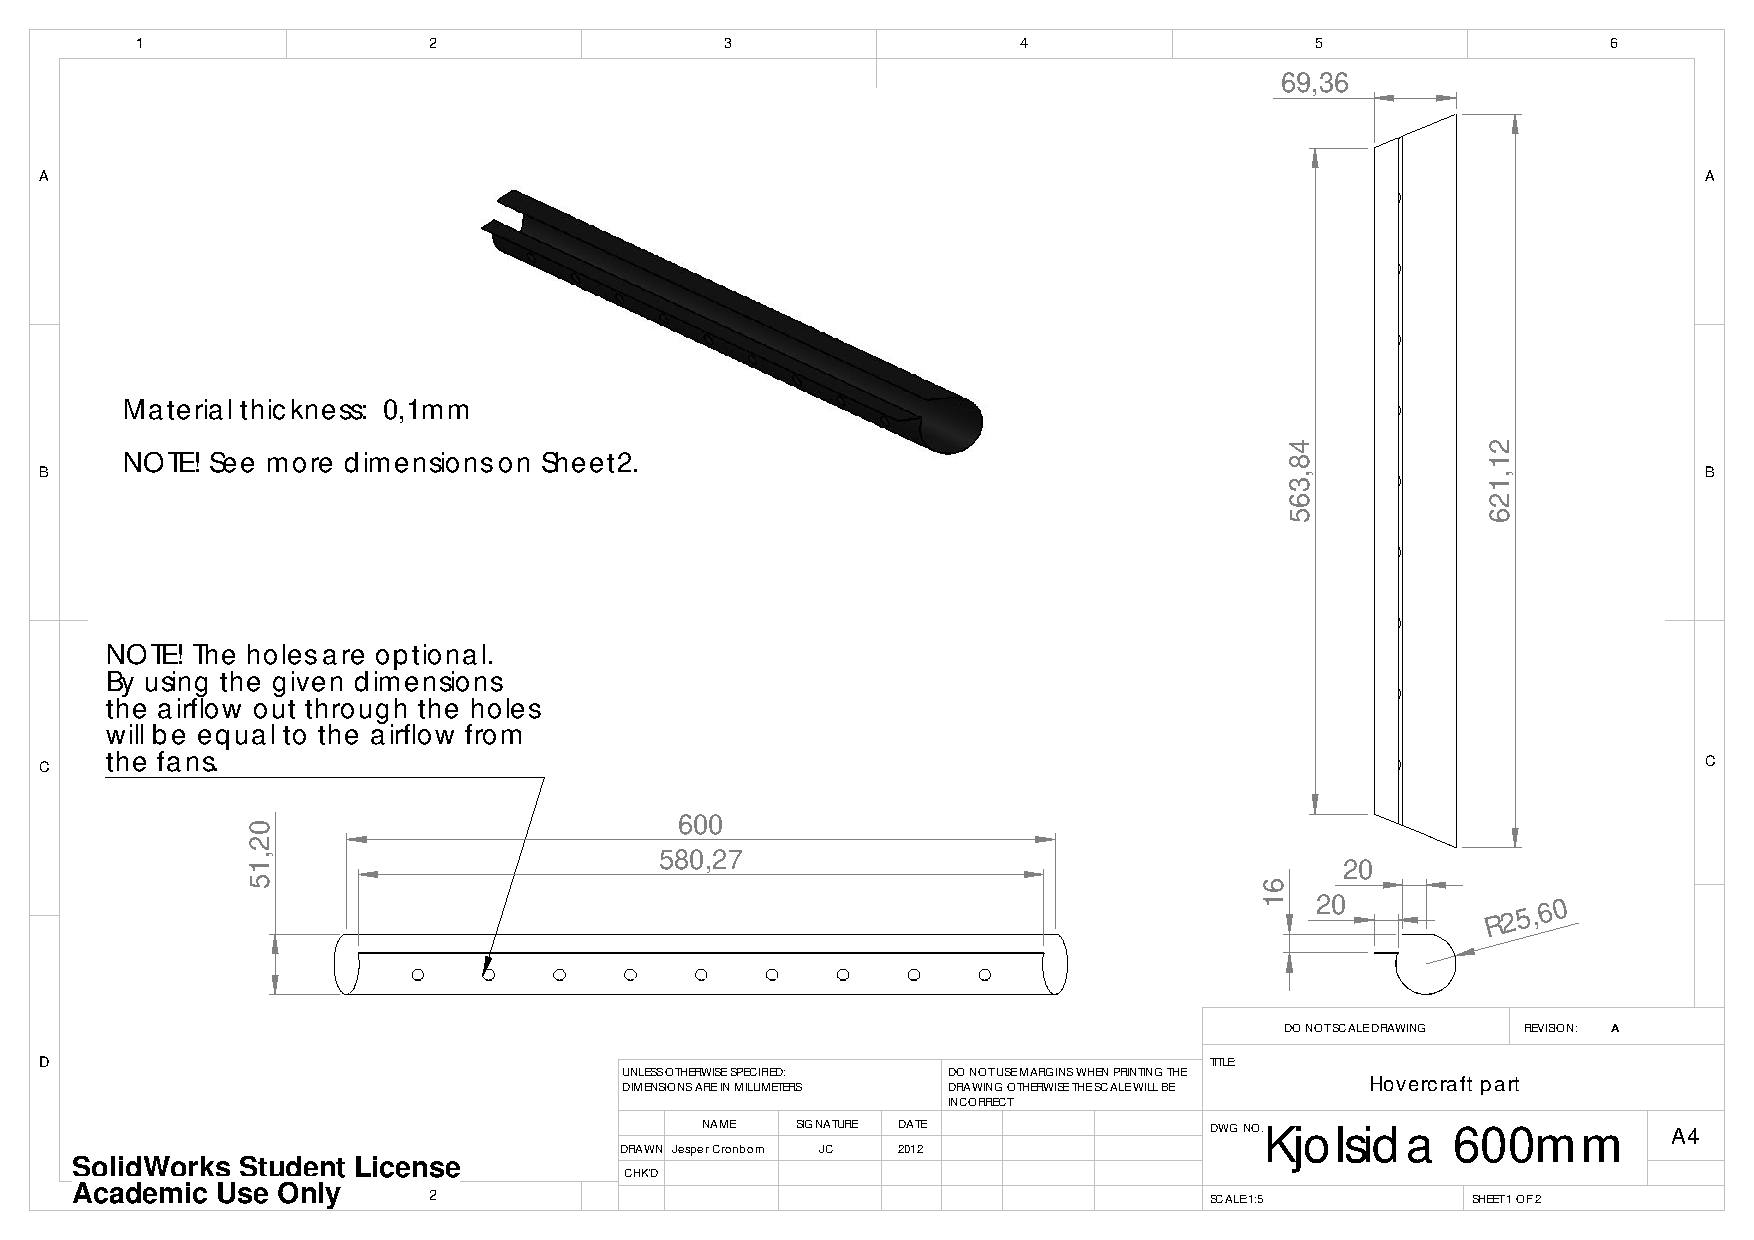
\includegraphics[width=18cm]{../../includes/figures/PDF_ritningar/Kjolsida_600}
\caption{Ritning över Kjolsida 600.}
\label{fig:Kjolsida_600}
\end{figure}
\end{landscape}

\begin{landscape}
\begin{figure}[htbp!]
\centering
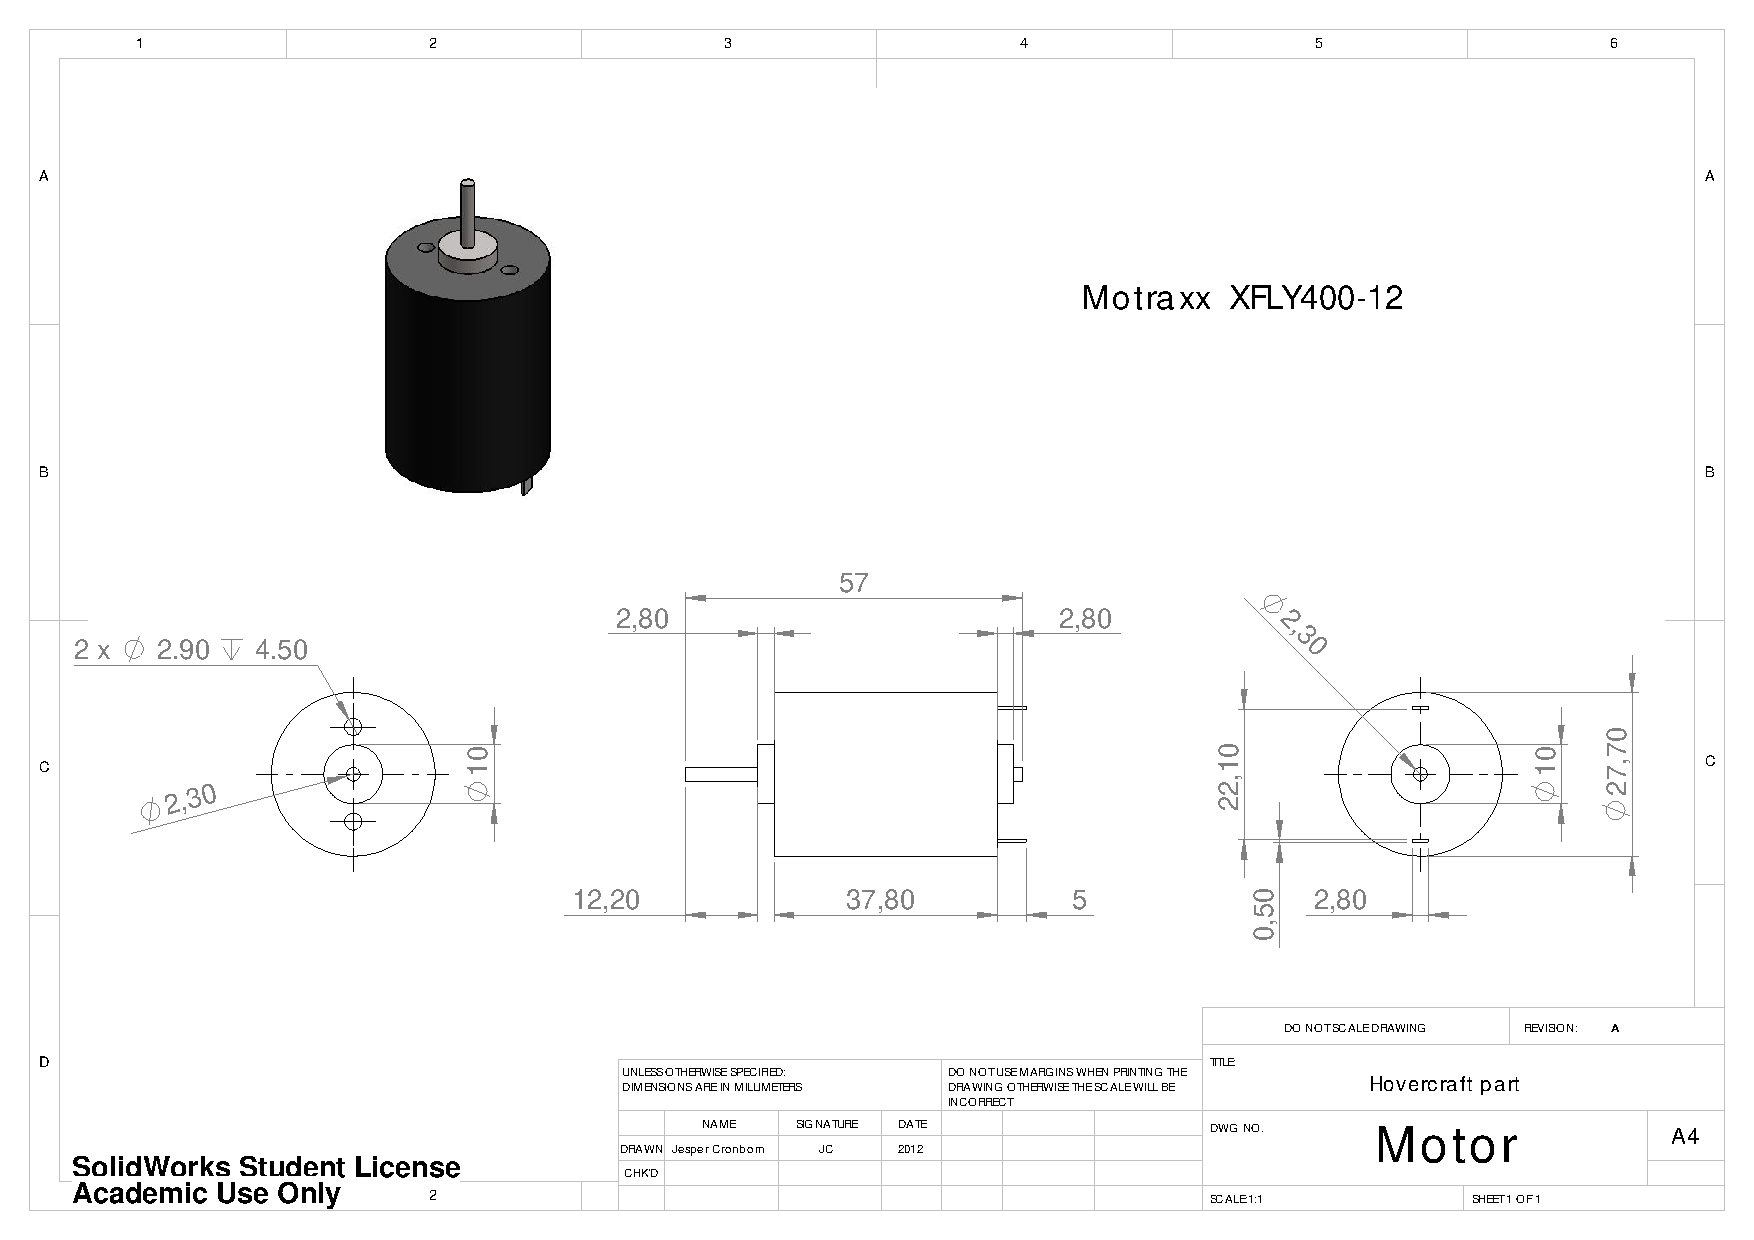
\includegraphics[width=18cm]{../../includes/figures/PDF_ritningar/Motor}
\caption{Ritning över motor.}
\label{fig:motor}
\end{figure}
\end{landscape}

\begin{landscape}
\begin{figure}[htbp!]
\centering
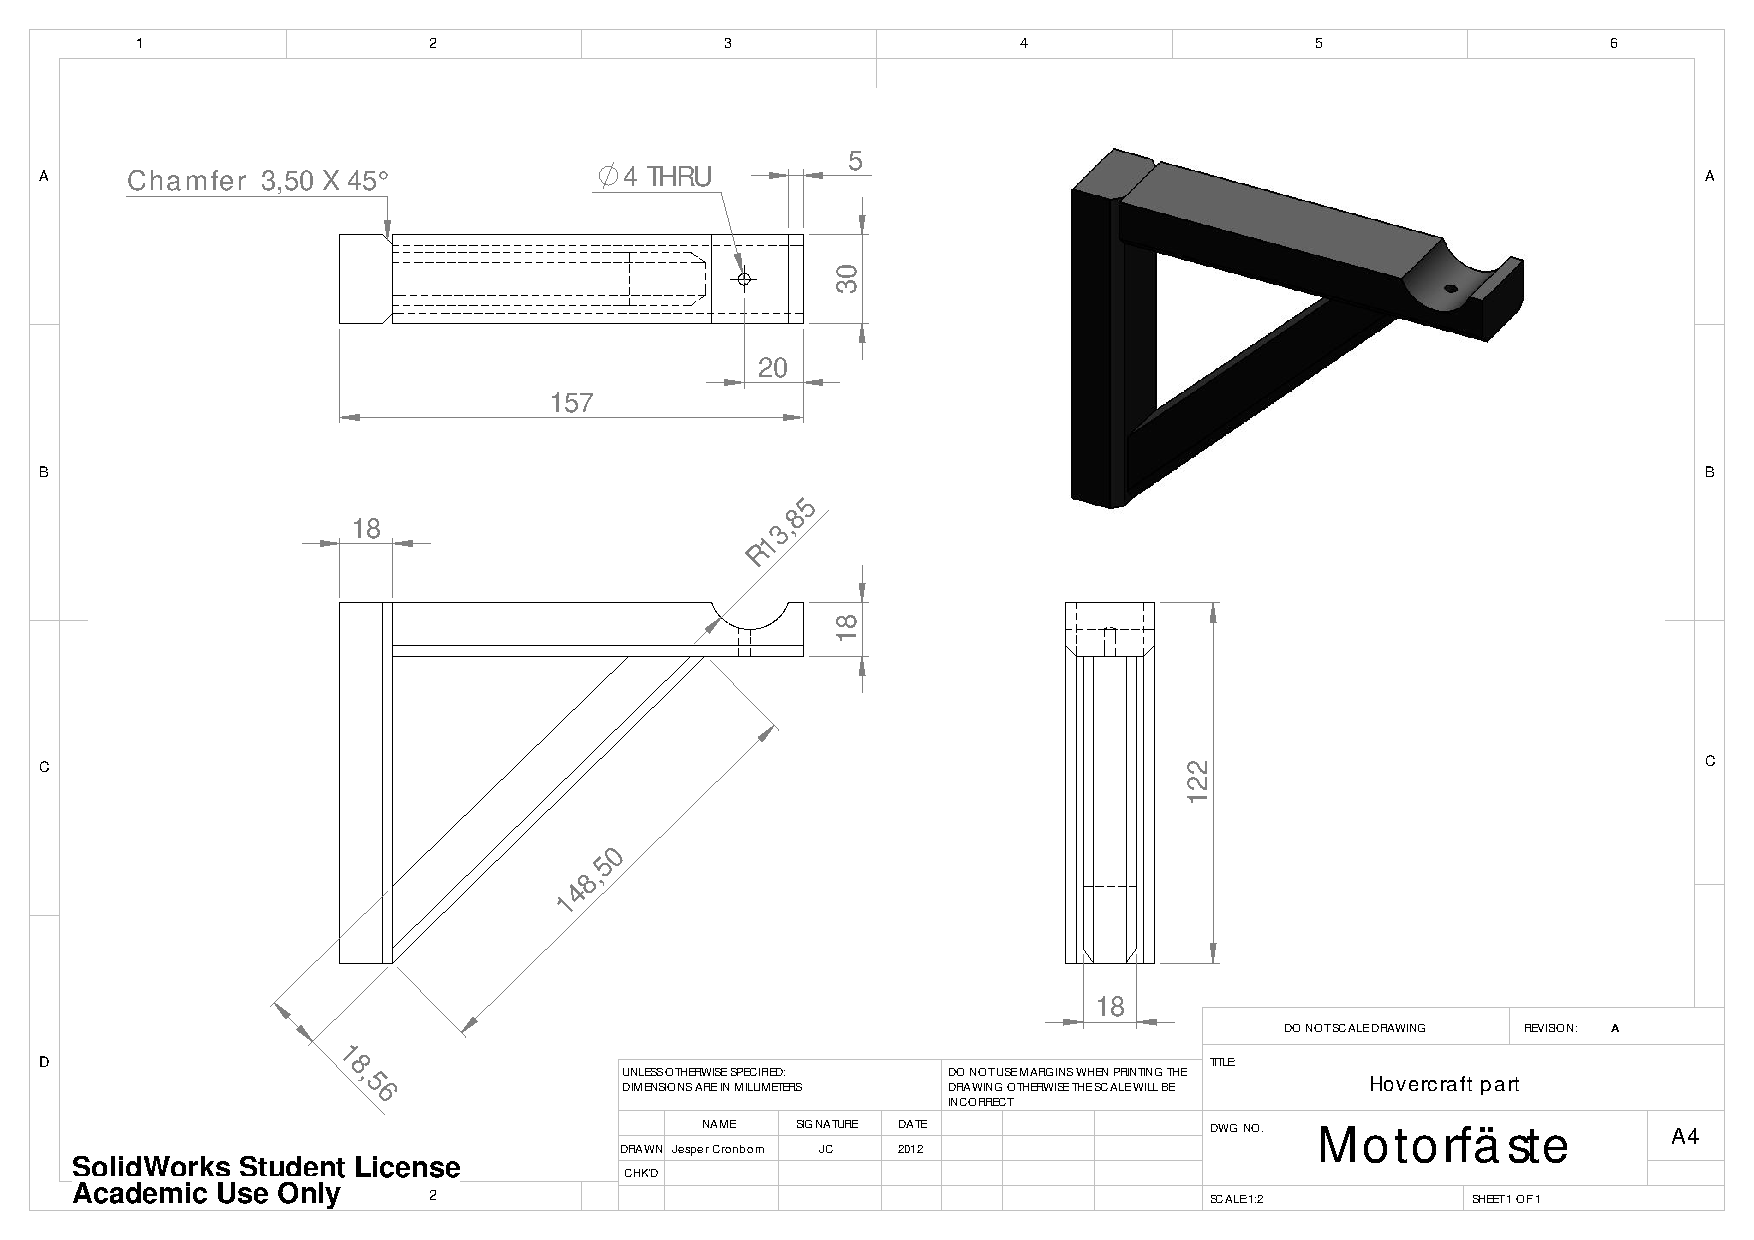
\includegraphics[width=18cm]{../../includes/figures/PDF_ritningar/Motorfaste}
\caption{Ritning över motorfäste.}
\label{fig:motorfaste}
\end{figure}
\end{landscape}

\begin{landscape}
\begin{figure}[htbp!]
\centering
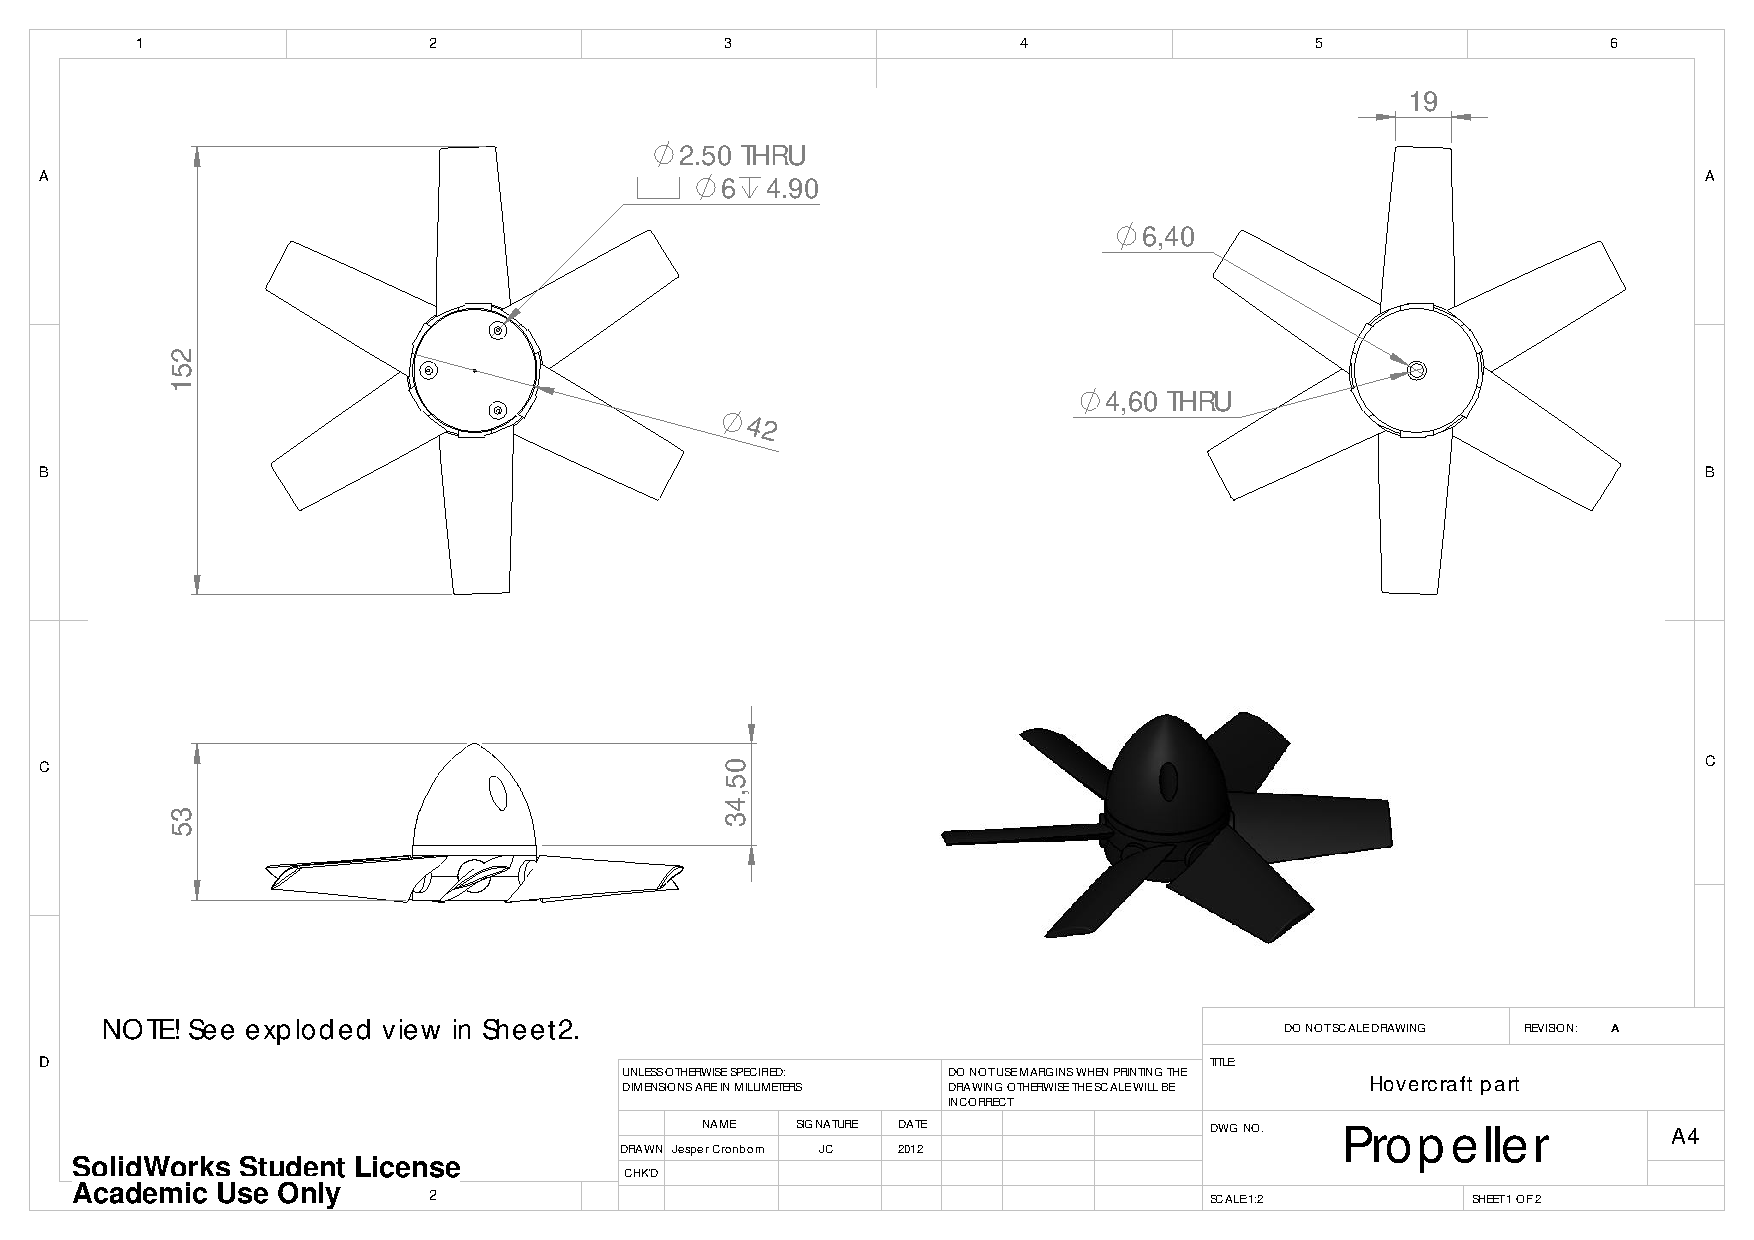
\includegraphics[width=18cm]{../../includes/figures/PDF_ritningar/Propeller}
\caption{Ritning över propeller.}
\label{fig:propeller}
\end{figure}
\end{landscape}

\begin{landscape}
\begin{figure}[htbp!]
\centering
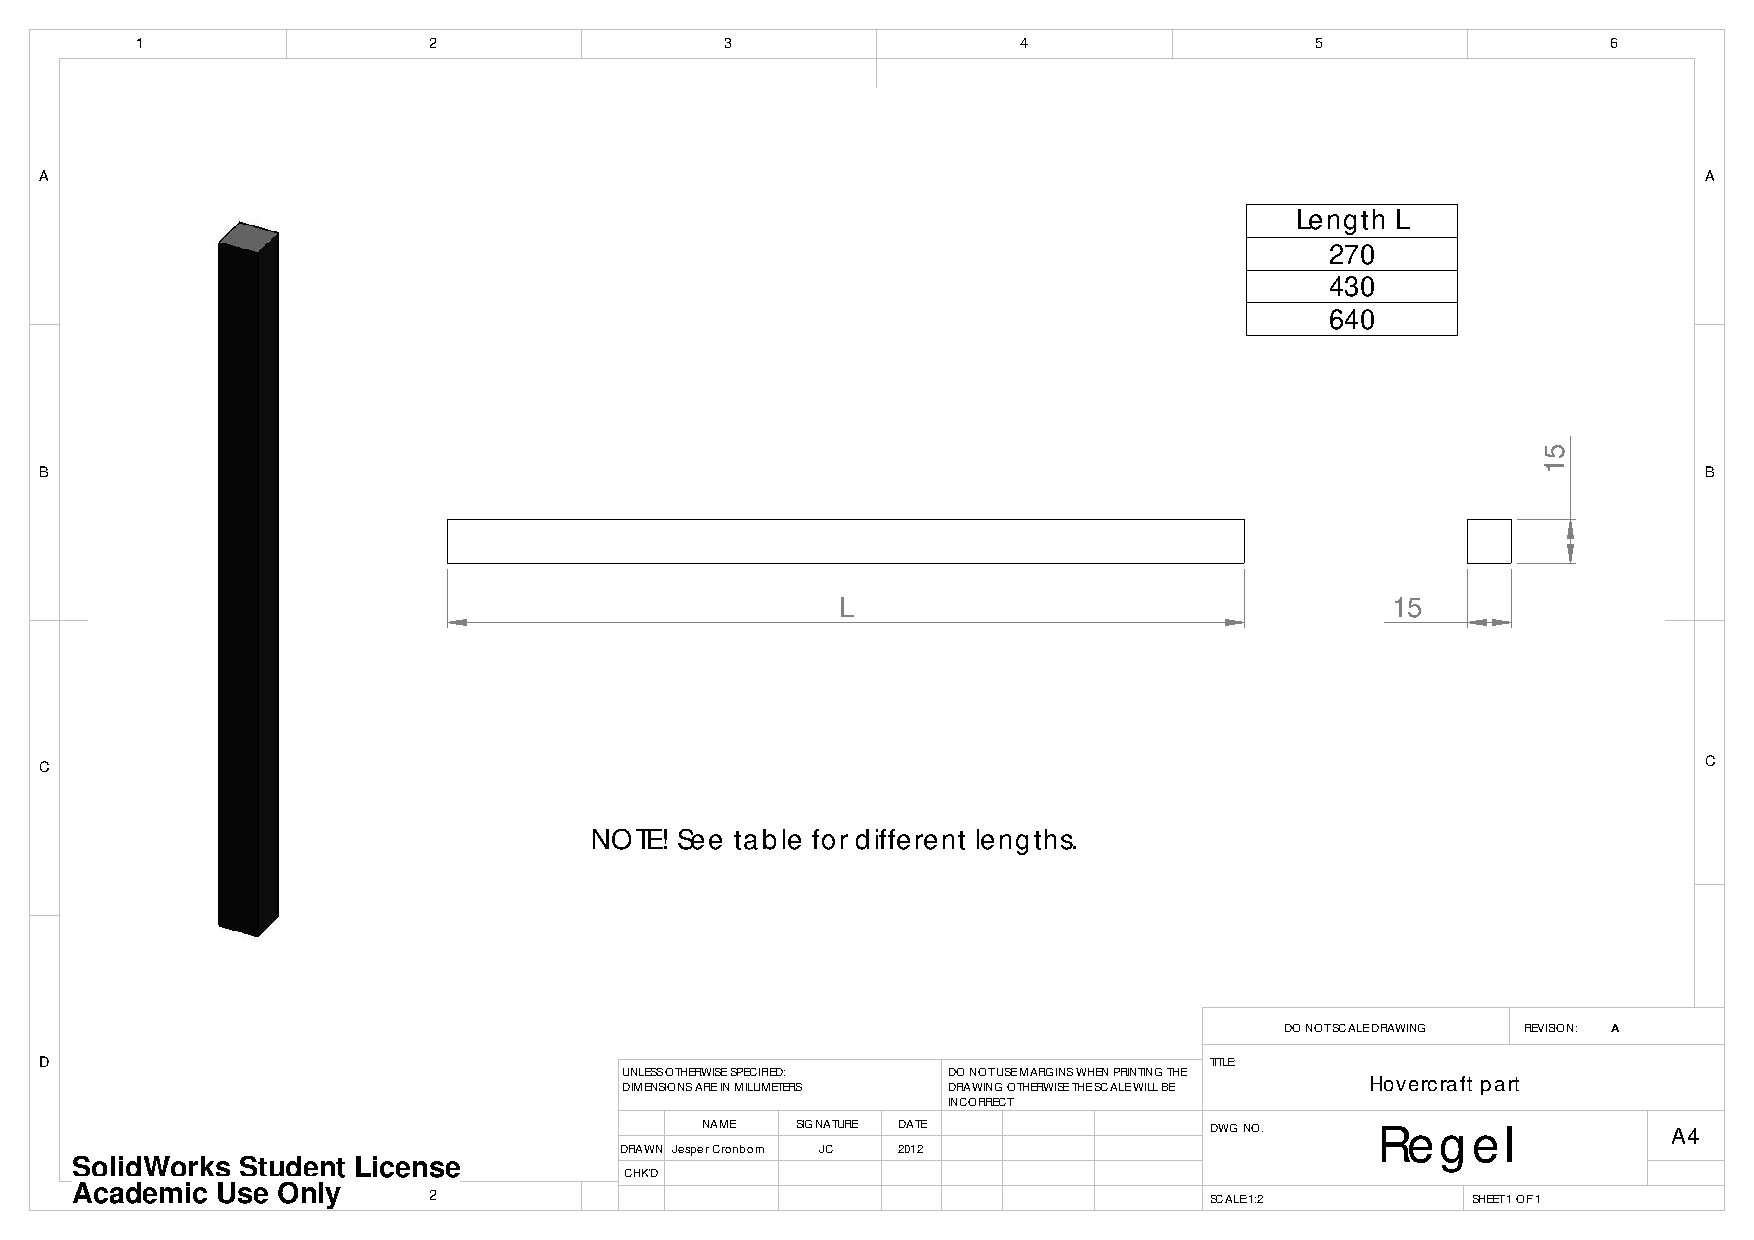
\includegraphics[width=18cm]{../../includes/figures/PDF_ritningar/Regel}
\caption{Ritning över regel.}
\label{fig:regel}
\end{figure}
\end{landscape}

\begin{landscape}
\begin{figure}[htbp!]
\centering
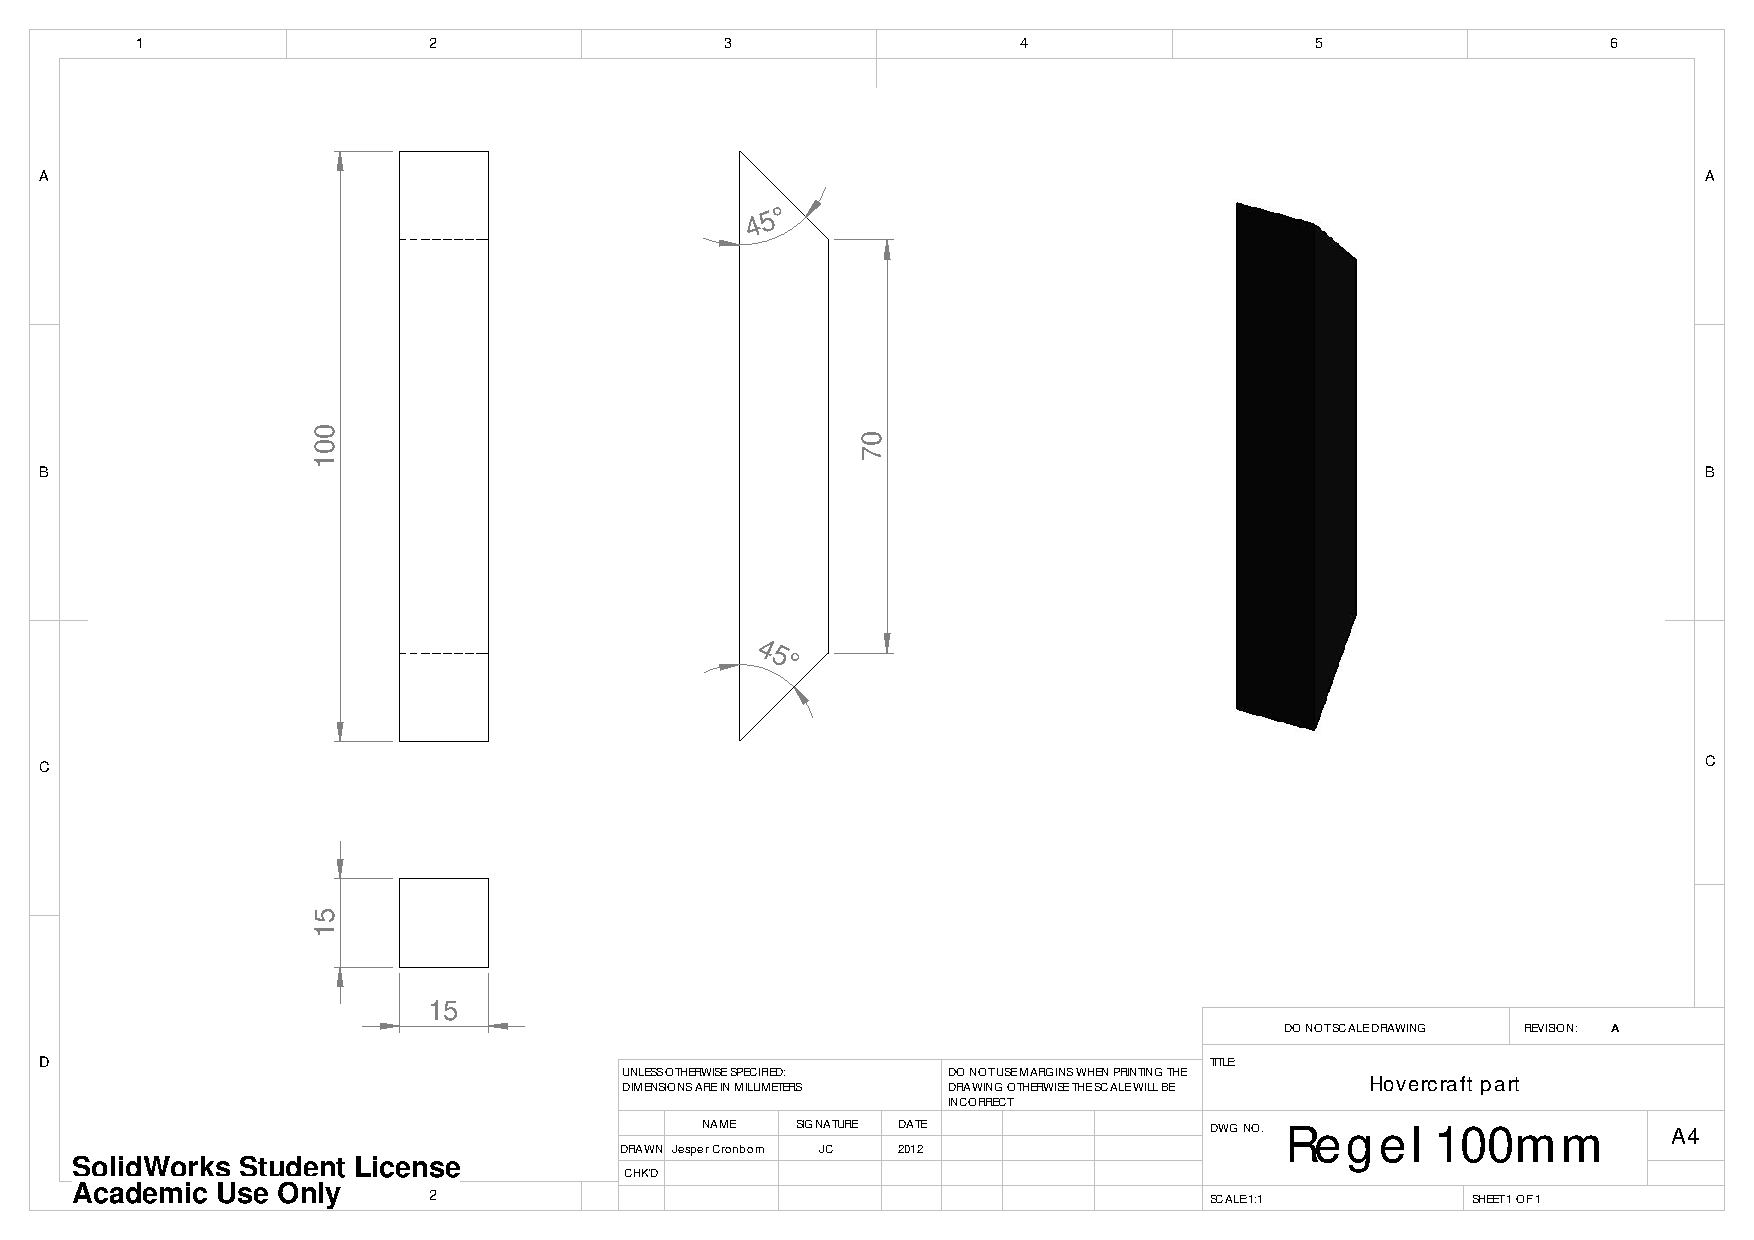
\includegraphics[width=18cm]{../../includes/figures/PDF_ritningar/Regel_100}
\caption{Ritning över regel 100.}
\label{fig:regel_100}
\end{figure}
\end{landscape}

\begin{landscape}
\begin{figure}[htbp!]
\centering
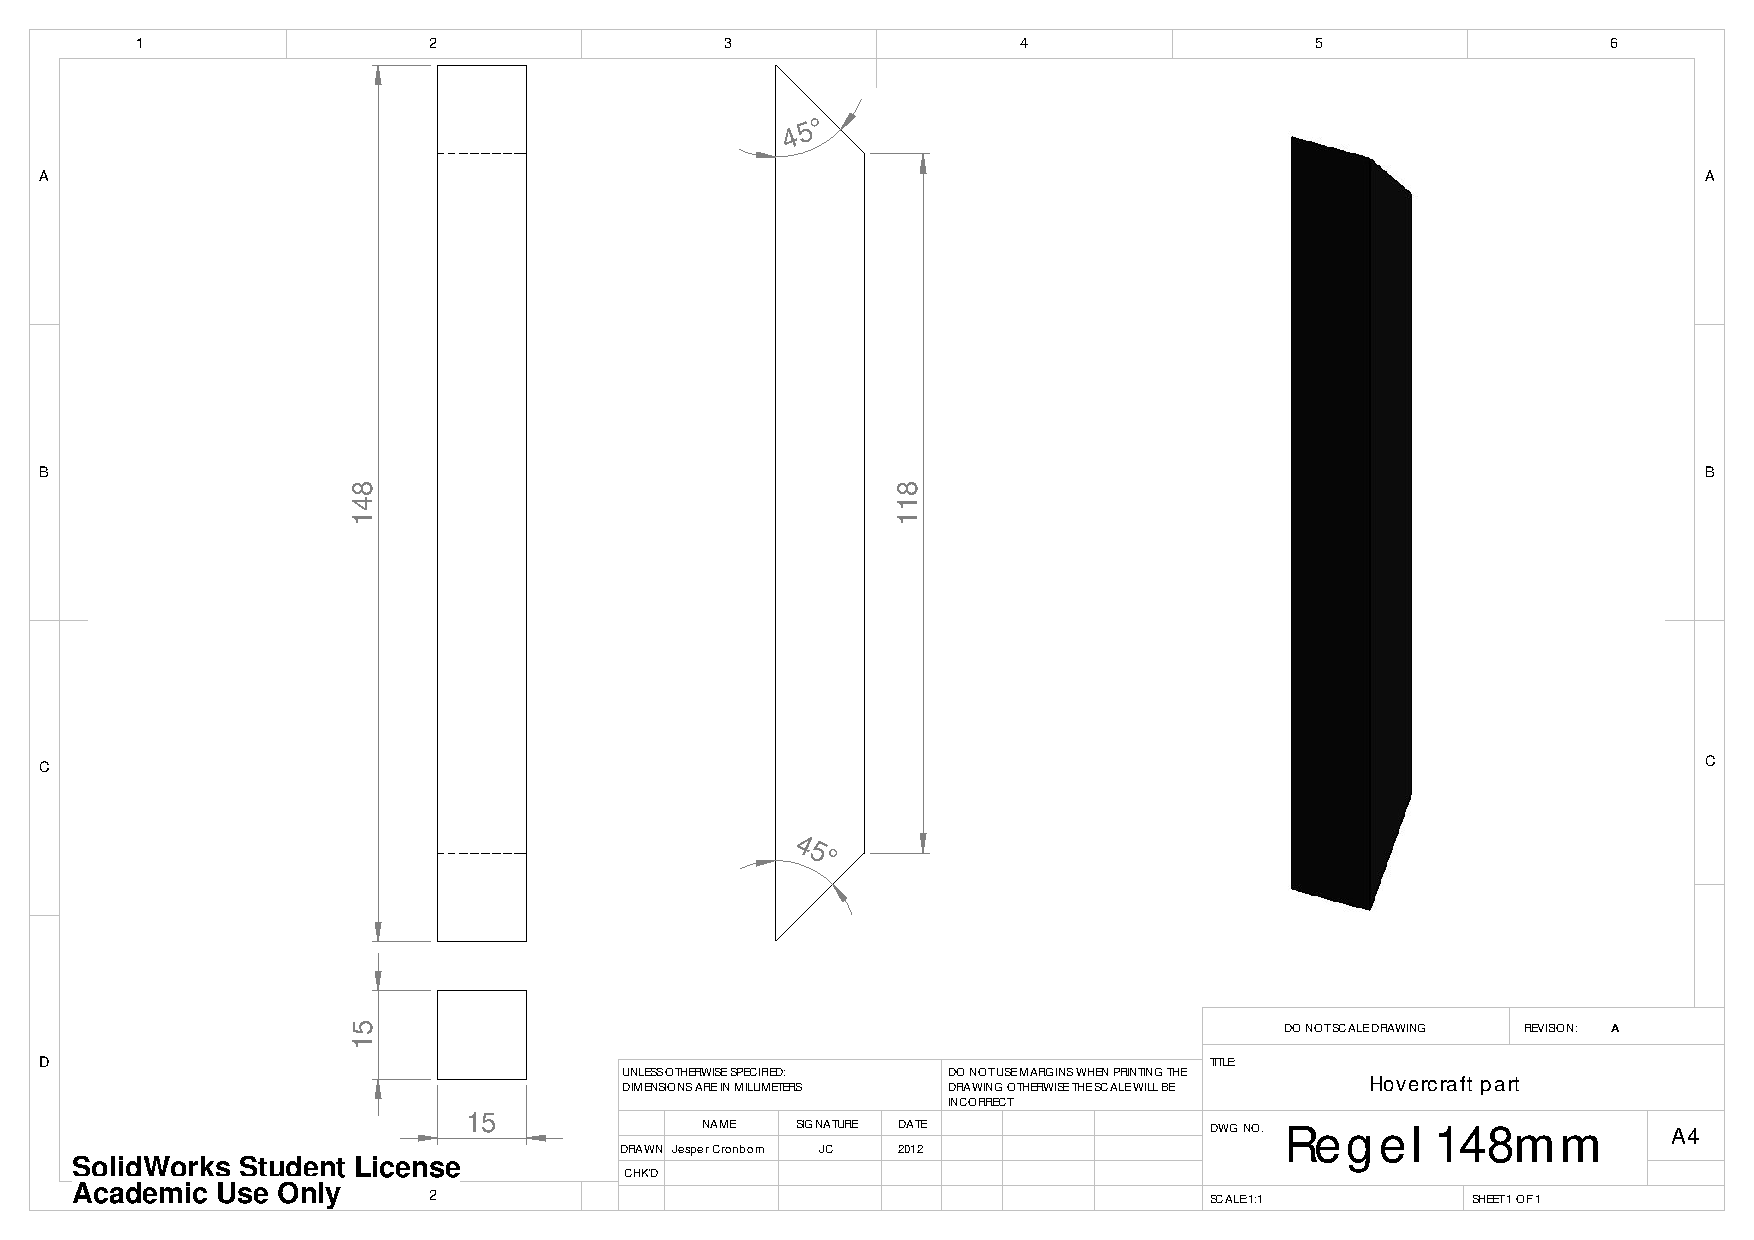
\includegraphics[width=18cm]{../../includes/figures/PDF_ritningar/Regel_148}
\caption{Ritning över regel 148.}
\label{fig:regel_148}
\end{figure}
\end{landscape}

\begin{landscape}
\begin{figure}[htbp!]
\centering
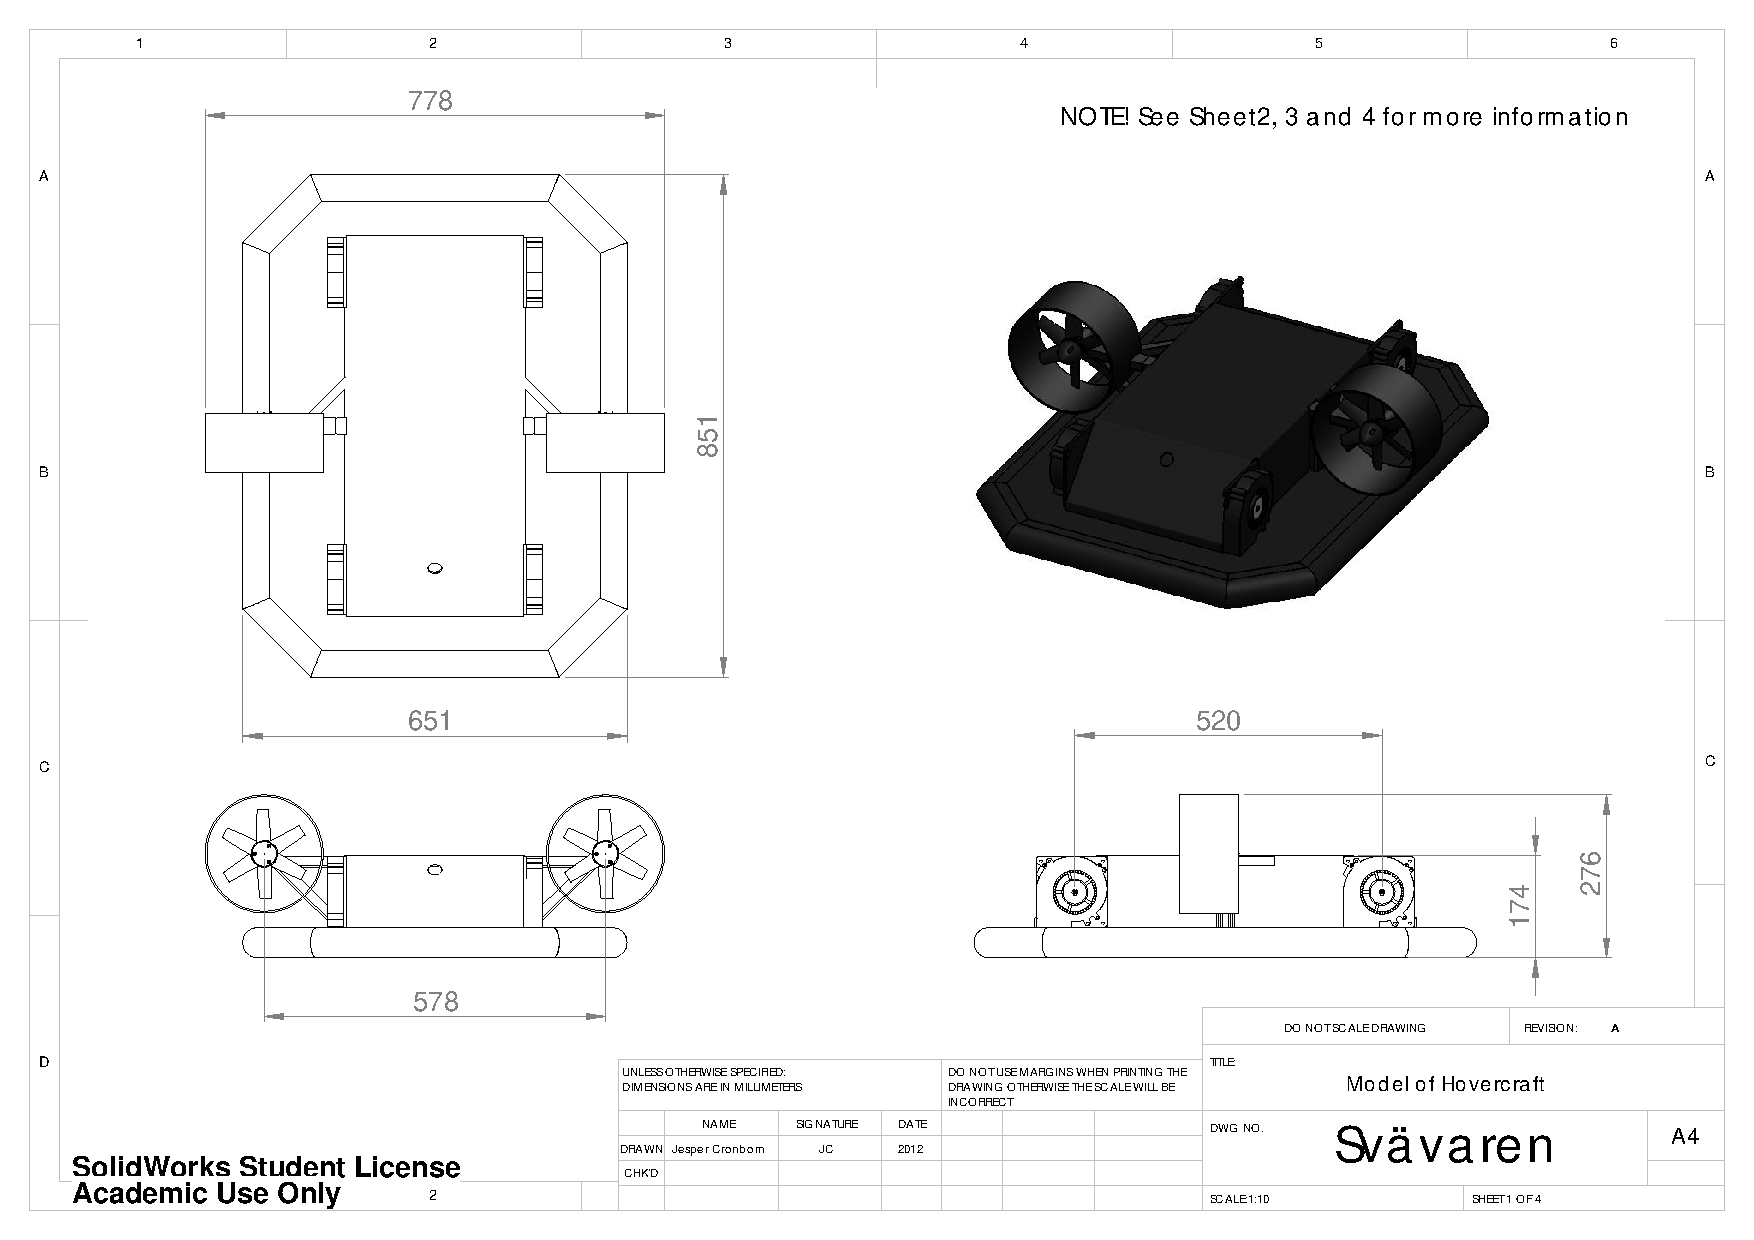
\includegraphics[width=18cm]{../../includes/figures/PDF_ritningar/Svavaren}
\caption{Ritning över svävaren.}
\label{fig:Svavaren_full}
\end{figure}
\end{landscape}

\begin{landscape}
\begin{figure}[htbp!]
\centering
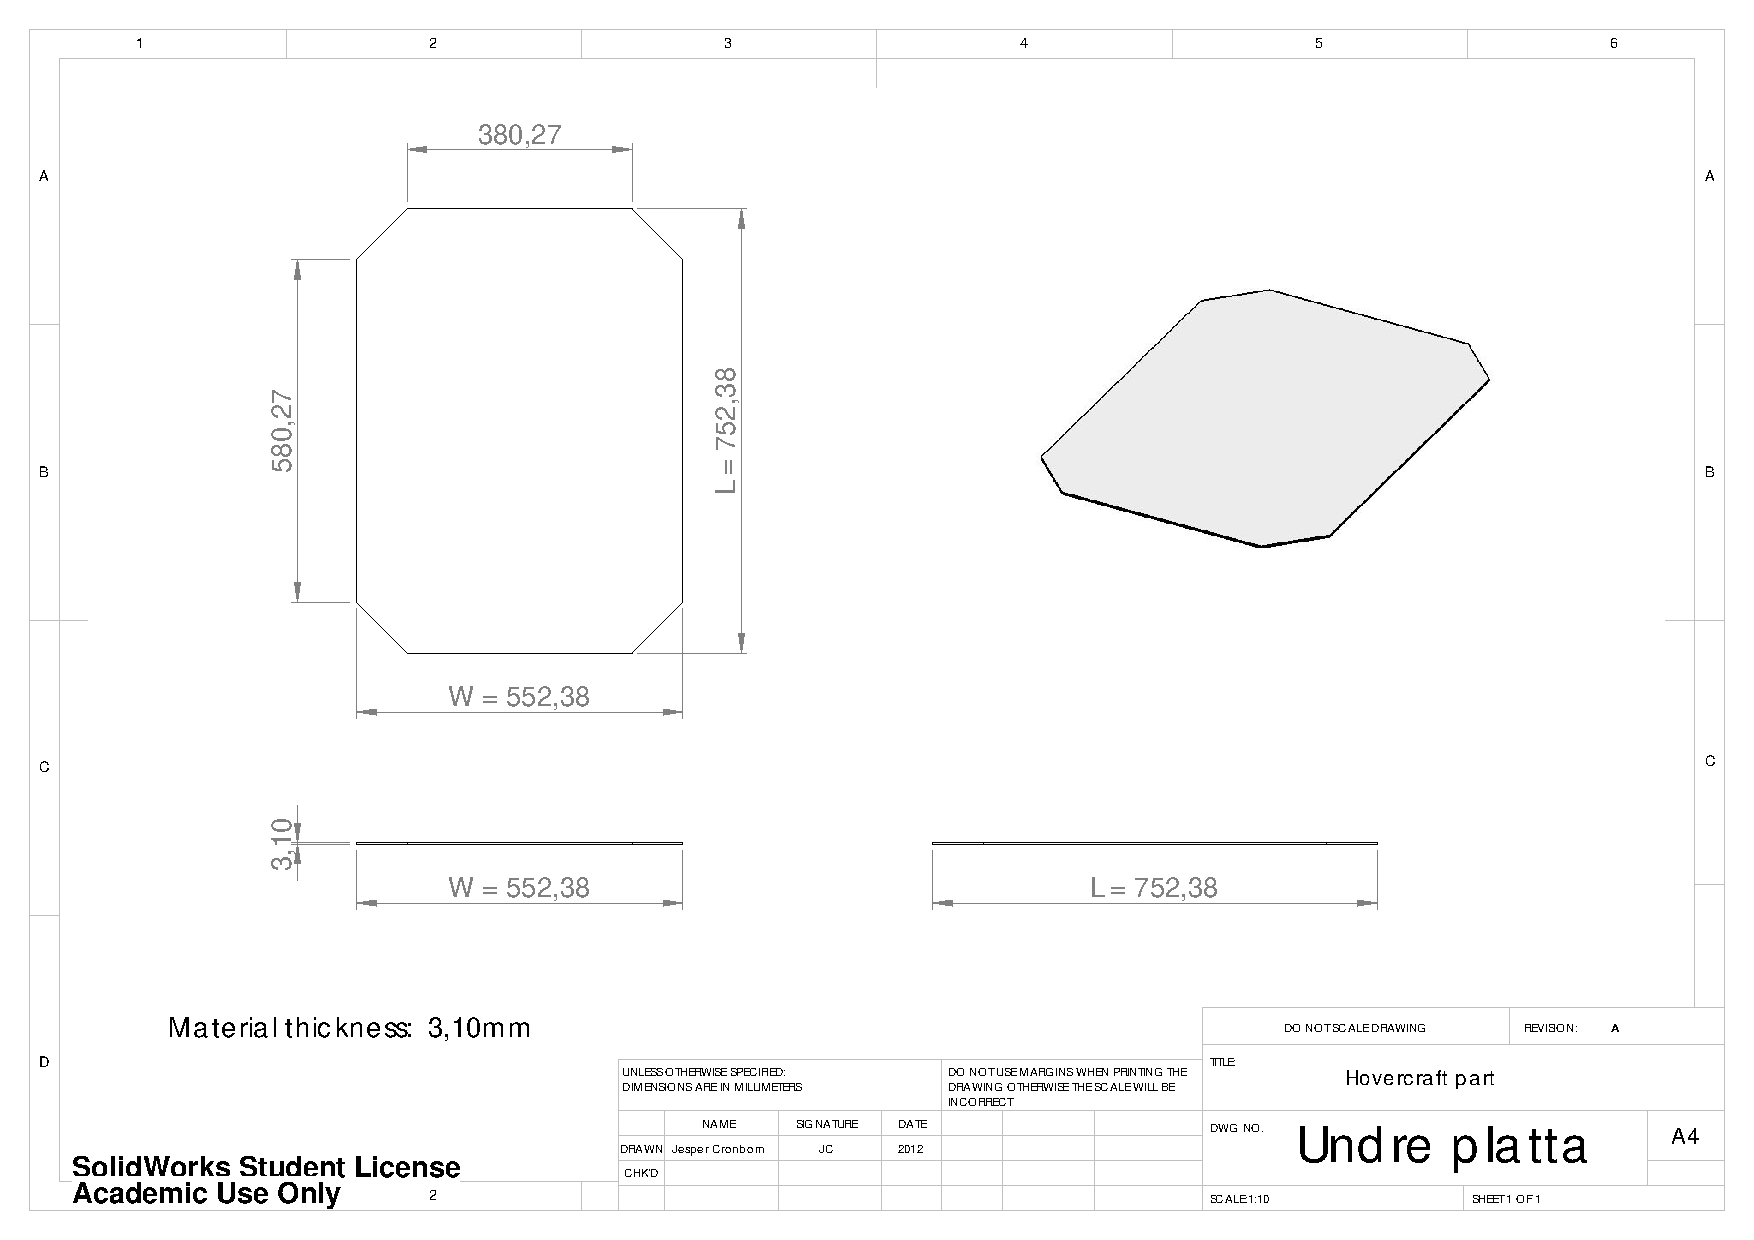
\includegraphics[width=18cm]{../../includes/figures/PDF_ritningar/Undre_platta}
\caption{Ritning över svävaren.}
\label{fig:Svavaren}
\end{figure}
\end{landscape}

\begin{landscape}
\begin{figure}[htbp!]
\centering
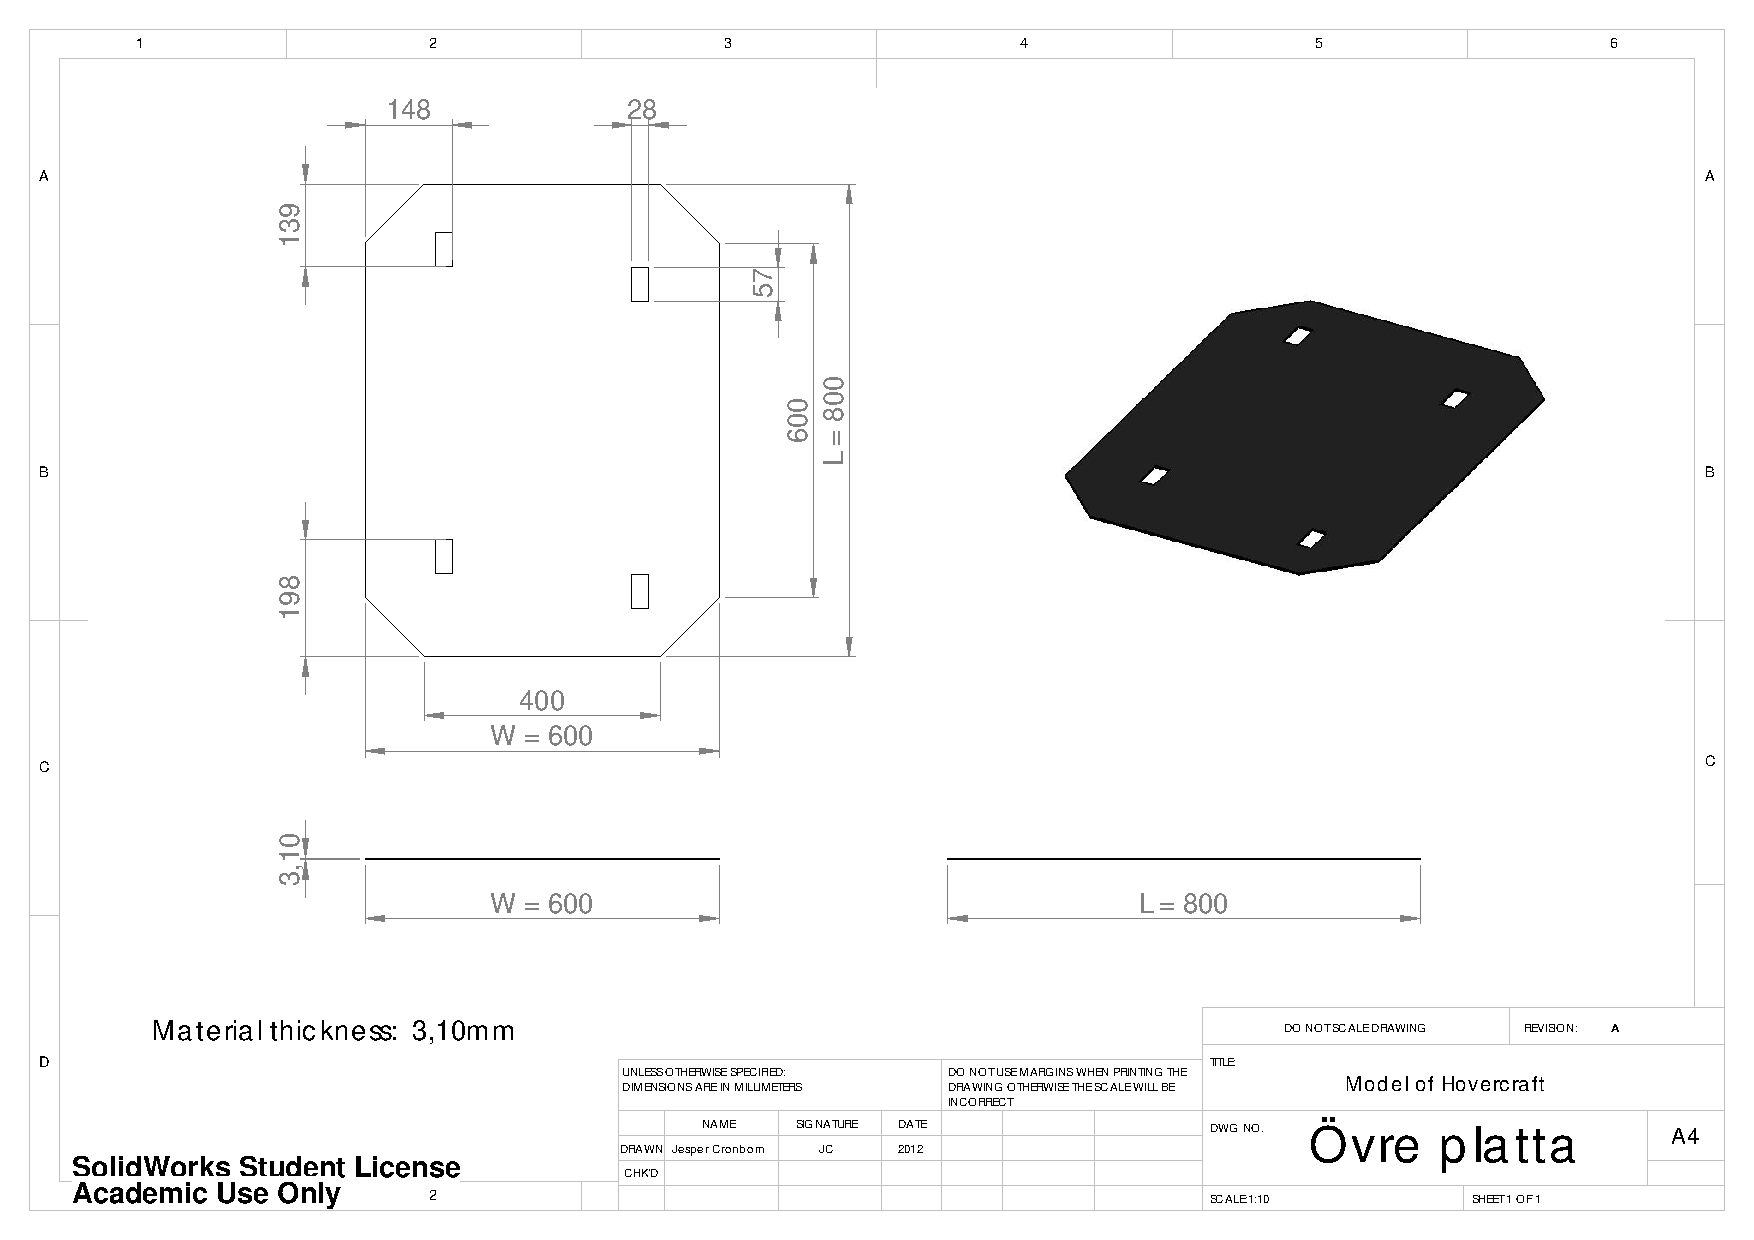
\includegraphics[width=18cm]{../../includes/figures/PDF_ritningar/Ovre_platta}
\caption{Ritning över övre plattan.}
\label{fig:Ovre_platta}
\end{figure}
\end{landscape}



\newpage
\section{Rapport H-brygga}
\label{apx:H-bridge}
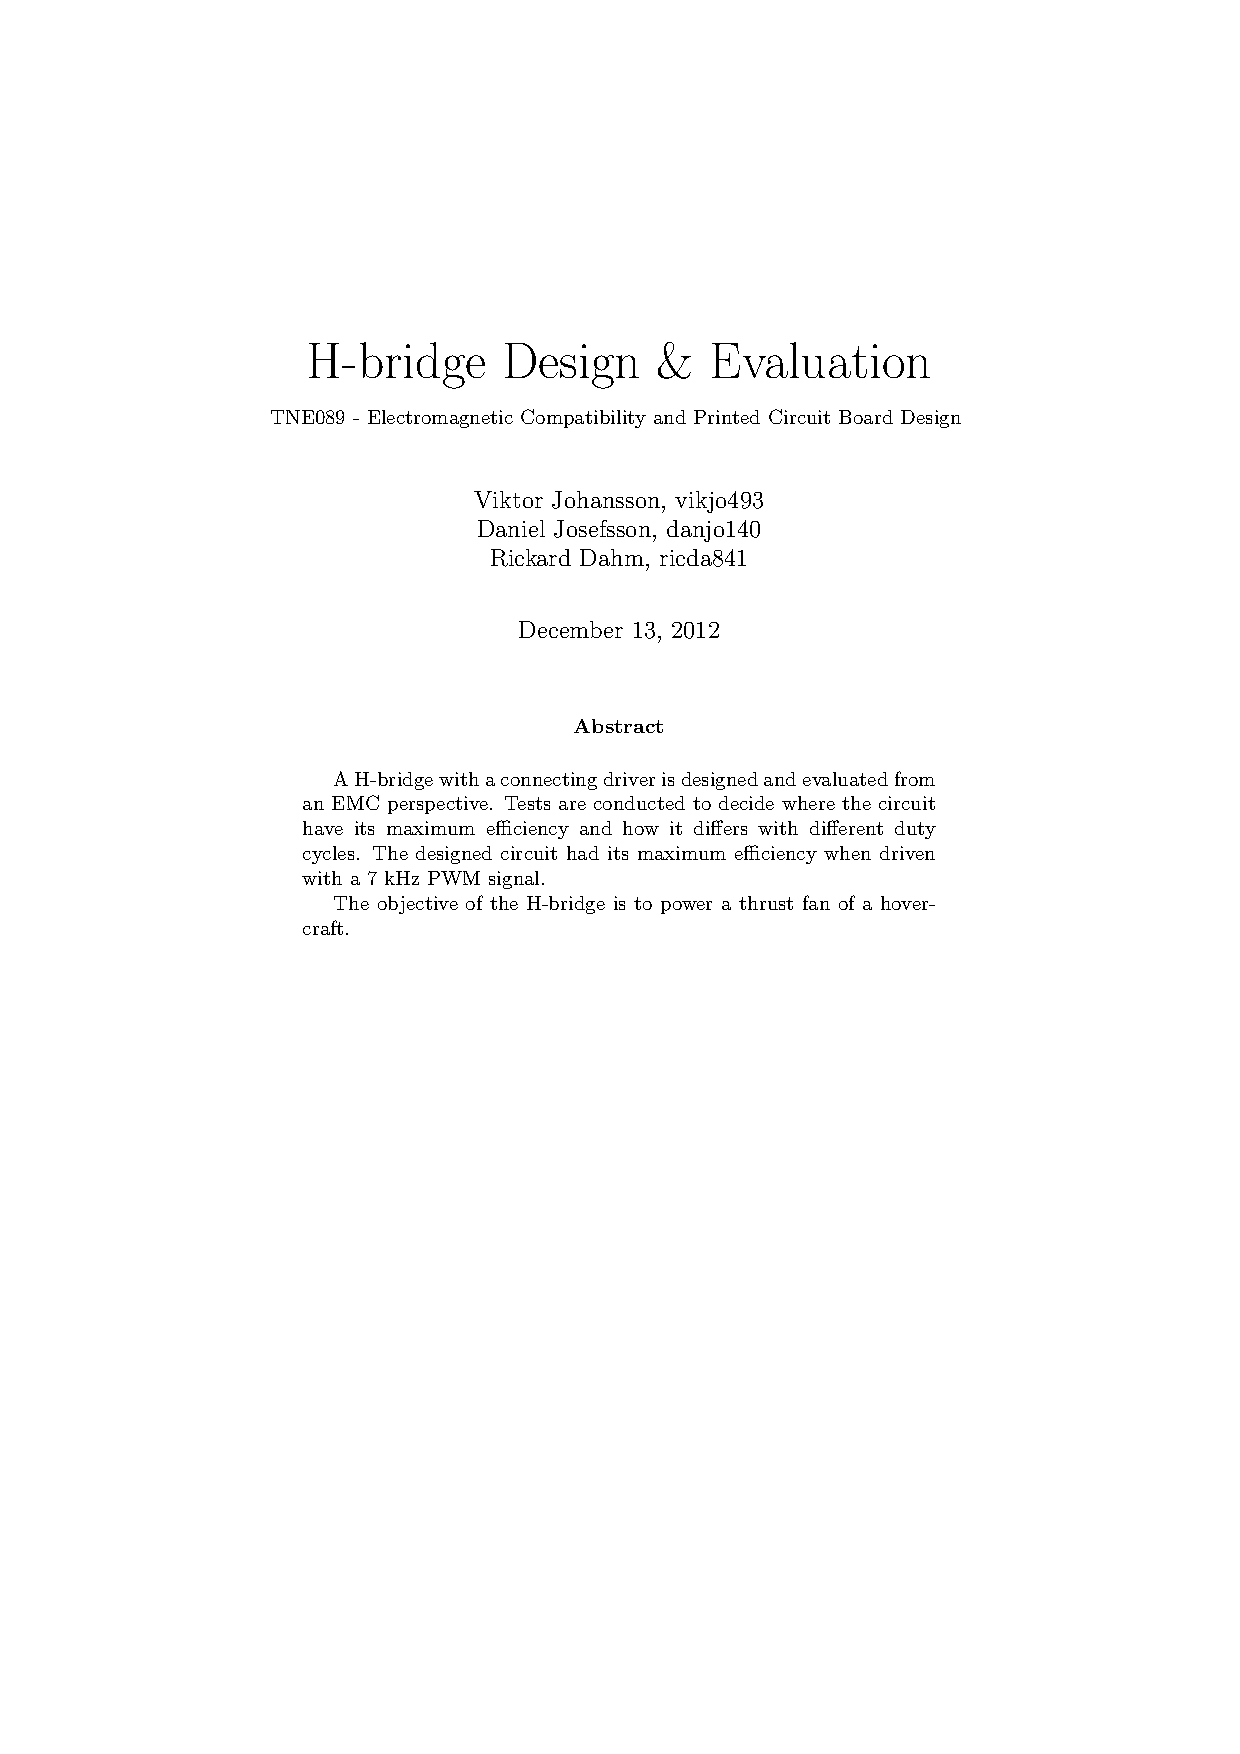
\includepdf[pages={-}]{appendix/TNE089-Project_Report_h_birdge.pdf}

\section{Rapport strömförsörjning}
\label{apx:PSU}
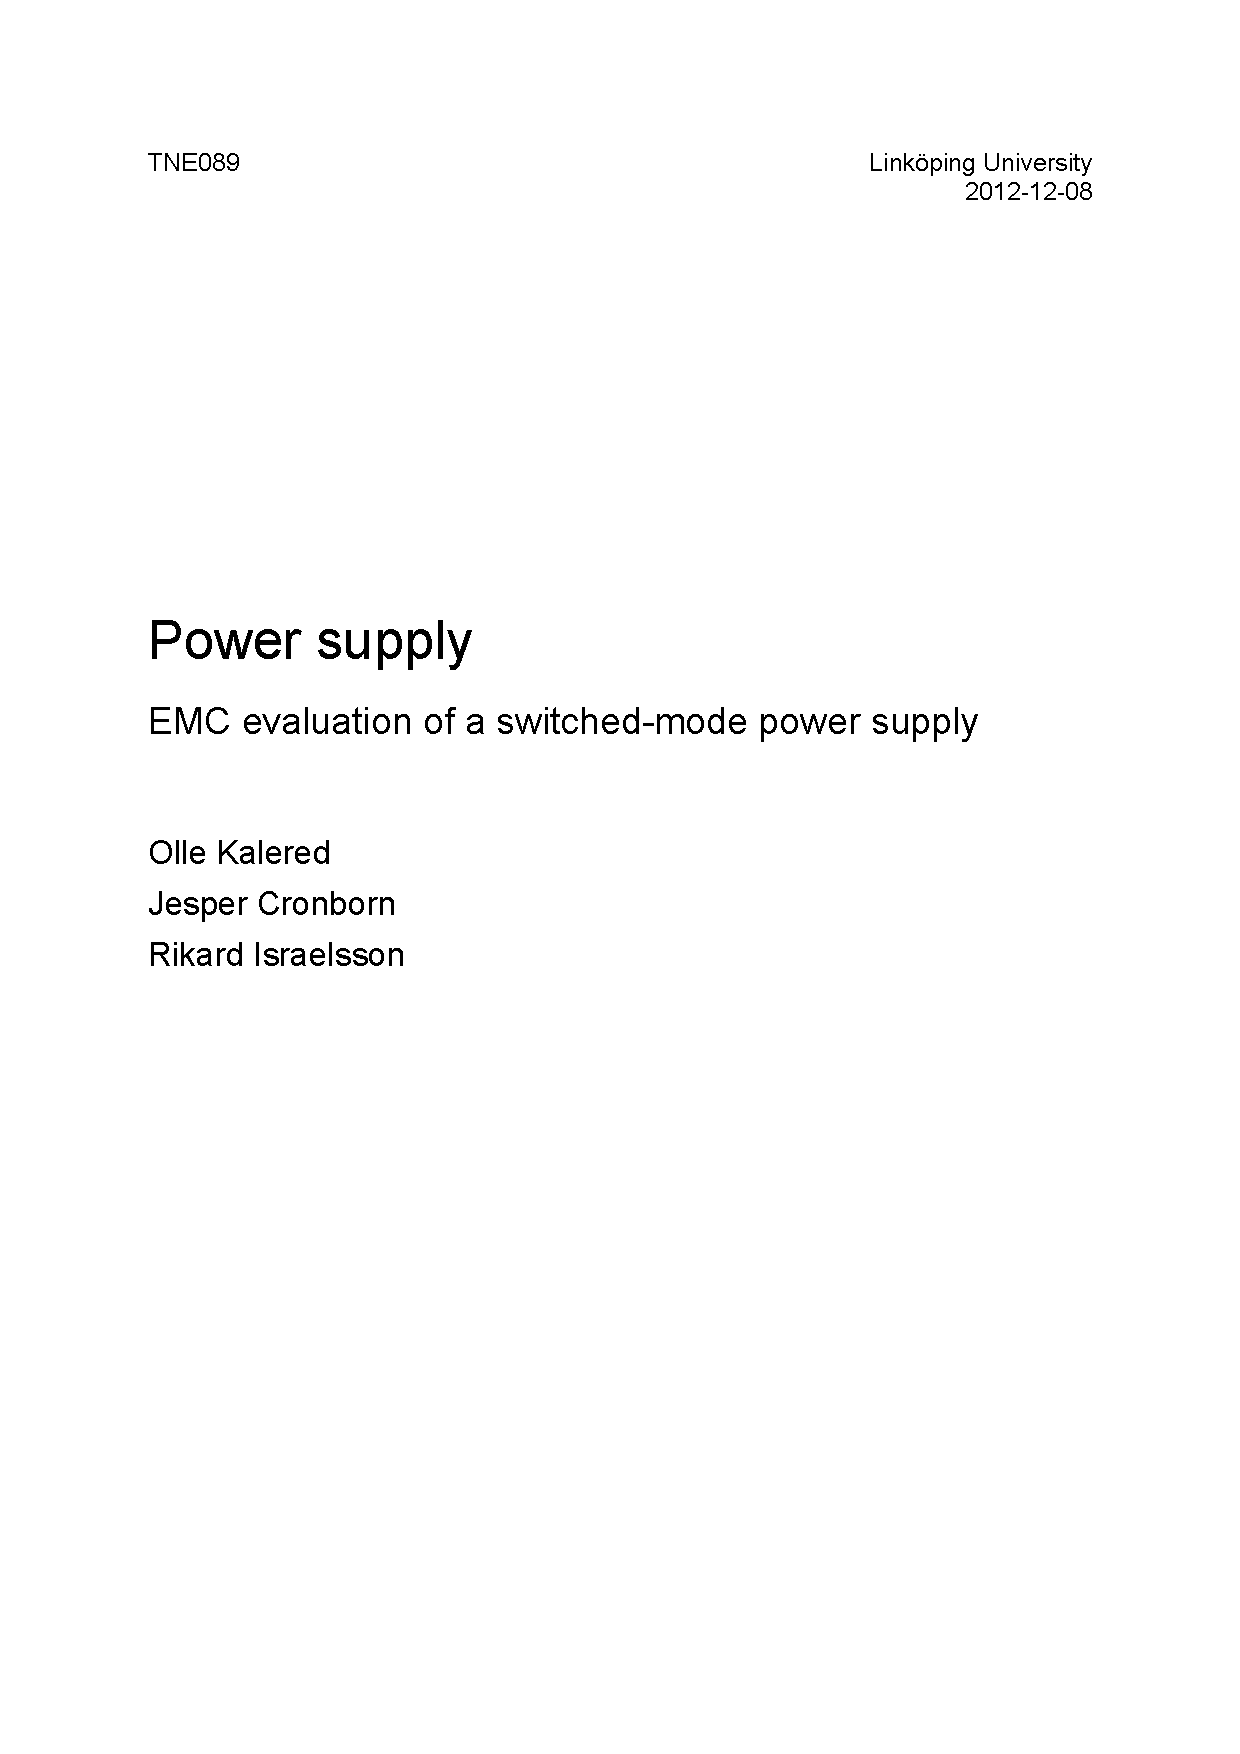
\includepdf[pages={-}]{appendix/TNE089-PowerSupplyReport.pdf}


\end{document}
